%____________________________________________________________________________||
\section{Event selection}
\label{sec:selection}

\subsection{Event vetoes for leptons, photons, and single isolated tracks\label{sec:vetoes}}

To suppress SM processes with genuine \met from neutrinos, events
containing an isolated electron with $\pt > 20\GeV$ and $|\eta| < 2.5$ or an isolated muon
with $\pt > 10\GeV$ and $|\eta| < 2.5$ are vetoed. To select a pure
multijet topology, events are vetoed in which an isolated
photon with $\pt > 25\GeV$ and $|\eta| < 2.5$ is
found.  Further, to reduce the ``lost leptons'' backgrounds from W~+~jets 
and \ttbar, events containing single isolated tracks with $\pt >
10\GeV$ and $|\eta| < 2.5$, as defined in
Section~\ref{sec:reconstruction}, are vetoed as part of the signal
region selection criteria. In the case of the \mj and \mmj
samples, a further requirement is made such that events are not vetoed
due to the presence of a track from the well identified muons, by
requiring $\Delta R(\textrm{track},\mu) < 0.02$.


%%____________________________________________________________________________||
\subsection{Hadronic region selection}

\subsubsection{Hadronic pre-selection}
Events are required to have significant hadronic activity by requiring
$\scalht > 200\GeV$. Despite the increase in centre of mass energy and pileup
in Run~2, this threshold is kept at the level of the Run~1 analyses~\cite{run1Analyses}  
to maintain acceptance for SUSY models with compressed spectra. This should be
made possible by the advances made in offline object reconstruction, particularly pileup
subtraction~\cite{puppi}.

Jets considered in the analysis are required to have an $\ET>40\gev$ and be
within the central tracker acceptance ($|\eta|<3.0$). This threshold is chosen
to be flat across \HT values, unlike the SUS-14-006 analysis. The \ET value is
chosen to be as low as possible to reduce the number of jets falling below
threshold and introducing artificial \mht, while remaining in the realm of
reliable jet energy corrections. In the nominal analysis the lead two jets 
are required to satisfy $\ET>100\gev$ and the lead jet must
have $|\eta|<2.5$. The jets that are accepted are used for the calculation of
the variables \HT and \mht.

Events in which jets with $\ET>40\gev$ are reconstructed with $|\eta|>3.0$ are
vetoed. This reduces the number of events with non genuine \mht caused by jets
just out of acceptance.

\subsubsection{The hadronic signal region\label{sec:had-signal}}

Following the hadronic pre-selection, the multijet background from QCD
is still several orders of magnitude larger than the typical signal
expected from SUSY. Most multijet background sits at $\alphat<0.5$ so can be 
rejected with very high efficiency by requiring an appropriate cut on this
variable (plus the application of two dedicated cleaning filters, described below in
Sec.~\ref{sec:had-signal}). As the mulitjet background is more prevalent at low
\HT values, an \alphat cut that scales with \HT is required, detailed in
Table~\ref{tab:alphat-thresholds}. The minimum \mht value that the \alphat cut
corresponds to is calculated by assuming $\dht=0$ and inverting the formula for
\alphat. The low \HT bins are most likely to be contaminated by QCD so the \alphat threshold 
is scaled up until the bin is QCD free. The value of \mht that this
approximately corresponds to is calculated and the \alphat cut for the
subsequent bins is chosen to keep this \mht approximately constant. As high 
\alphat cuts can have a significant effect on signal acceptance, it is
advantageous to tune the cut to maintain a high signal to background ratio while 
remaining QCD free.

\begin{table}[h!]
  \caption{\alphat and (effective) \mht thresholds per \scalht bin.\label{tab:alphat-thresholds}}
  \centering
  \footnotesize
  \begin{tabular}{ lcccccc }
    \hline
    \hline
    \scalht bin  & 200--250   & 250--300   & 300--350  & 350--400  & 400--900  & $>$900       \\
    \hline                                                                     
    \alphat      & 0.65       & 0.60       & 0.55      & 0.53      & 0.52      & 0.505         \\
    "Min \mht"   & $\sim$128  & $\sim$138  & $\sim$125 & $\sim$133 & $\sim$137 & $\gtrsim$126 \\
    \hline
    \hline
  \end{tabular}
\end{table}

In the Run~1 analyses there was a minimum cut of $\alphat>0.55$. This was chosen
as a conservative cut to remove QCD. It was also required
by the \alphat requirement in the HLT paths used to seed the analysis bins. For
Run~2 it is proposed to seed the the bins with $\HT>900\gev$ by a flat
$PF\HT>900\gev$ HLT path with no \alphat requirement.

Subsequently, additional cleaning cuts are applied. To protect against 
multiple jets failing the $\Et$ threshold, the
jet-based estimate of the missing transverse energy, \mht, is compared
to the Particle Flow estimate of missing transverse energy, $\pfmet$,
and events with $R_{\rm miss}=\mht/\pfmet > 1.25$ are rejected.

To protect against severe energy losses, events with significant jet
mismeasurements caused by masked regions in the ECAL (which amount to
about 1\% of the ECAL channel count), or by missing instrumentation in
the barrel-endcap gap, are removed with the following procedure. The
jet-based estimate of the missing transverse energy, \mht, is used to
identify jets most likely to have given rise to the \mht as those
whose momentum is closest in $\phi$ to the total $\vec{\mht}$ which
results after removing them from the event.  The azimuthal distance
between this jet and the recomputed \mht is referred to as
$\Delta\phi^*$ in what follows. Events with $\Delta\phi^* < 0.5$ are
rejected if the distance in the ($\eta,\phi$) plane between the
selected jet and the closest masked ECAL region, $\Delta R_{\rm
  ECAL}$, is smaller than 0.3. Similarly, events are rejected if the
jet points within 0.3 in $\eta$ of the ECAL barrel-endcap gap at
$|\eta| = 1.5$. These final selections complete the definition of the
acceptance of the hadronic signal sample.

%%____________________________________________________________________________||
\subsection{Analysis bins}

Events in the hadronic signal region (and the
three control regions described in Sec.~\ref{sec:controlSelection}) are
categorised according to the number of jets (\njet) reconstructed in
each event and the number of jets identified as originating from
bottom quarks (\nb) in each event. By construction, $\nb \leq \njet$.

Additionally these categories are split up into \HT bins, detailed in 
Table~\ref{tab:htBins}.
%HT bins table

% Introduce 2012 bins?

\subsubsection{Introduction of asymmetric jet bin}

% introduction of asymmetric dijet bin, describe the bin and small motivation

PLACEHOLDER: plot of njet for signal model, DM yield table?

\subsubsection{Extension of \HT bins}

\subsubsection{Fine \njet binning}

%%____________________________________________________________________________||
\subsection{Key distributions for the hadronic signal
  region\label{sec:mc-data-comp}}

PLACEHOLDER: plots of alphaT for signal region, HT, MHT, njet


%%____________________________________________________________________________||
\subsection{Breakdown of SM backgrounds in the hadronic signal
  region\label{sec:bkgd-comp}}

In the absence of multijet events from QCD, the remaining significant
backgrounds in the signal region are expected to stem from SM
processes with genuine \met in the final state. For the low jet
multiplicity categories, the largest backgrounds with genuine \met are
generally from the associated production of W or Z bosons with jets,
followed by either the weak decays \znunu\ or \wtaunu, where the
$\tau$ decays hadronically and is identified as a jet, or by leptonic
decays that are outside acceptance or not rejected by the dedicated
electron or muon vetoes. For the higher jet multiplicity categories,
top quark production followed by semileptonic weak top quark decay
becomes important. The relative contribution from \ttbar is enhanced
or suppressed depending on the number of b-jets required. 
% A breakdown
% of the relative contributions of the SM backgrounds, as given by
% simulation, in the different (\njet, \nb, \scalht) bins can be found
% in Table~\ref{tab:backgrounds}. 
A plot showing the yields for these electroweak backgrounds and a reference
signal model can be seen in Fig~\ref{fig:ewkYields}

\begin{figure}[h!]
  \centering
  \subfigure[Hadronic signal region yields for electroweak backgrounds
  ($\njet = 2$)]{
    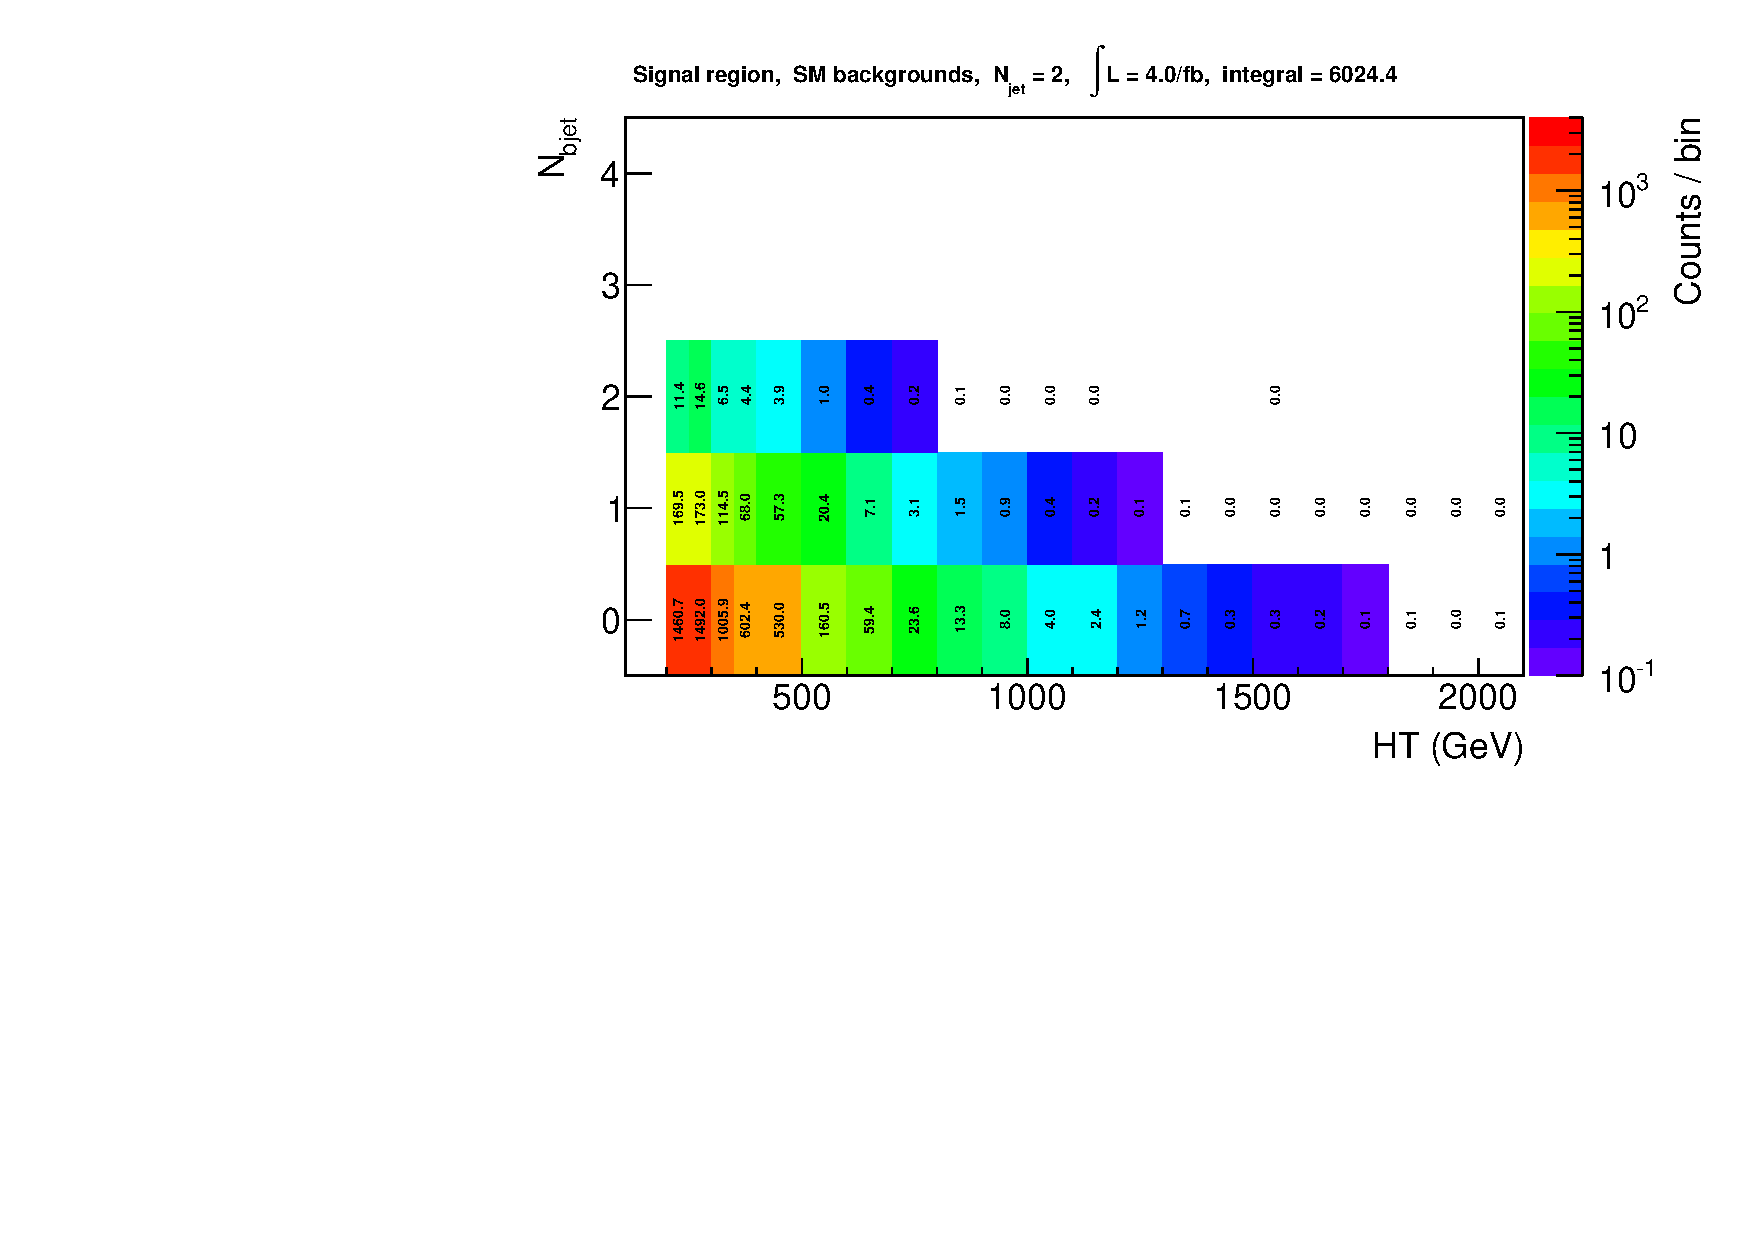
\includegraphics[width=0.5\textwidth]{figures/yieldPlots/had_ewk_eq2j.pdf}
  }~~
  \subfigure[Hadronic signal region yields for the \zinv background
  ($\njet = 2$)]{
    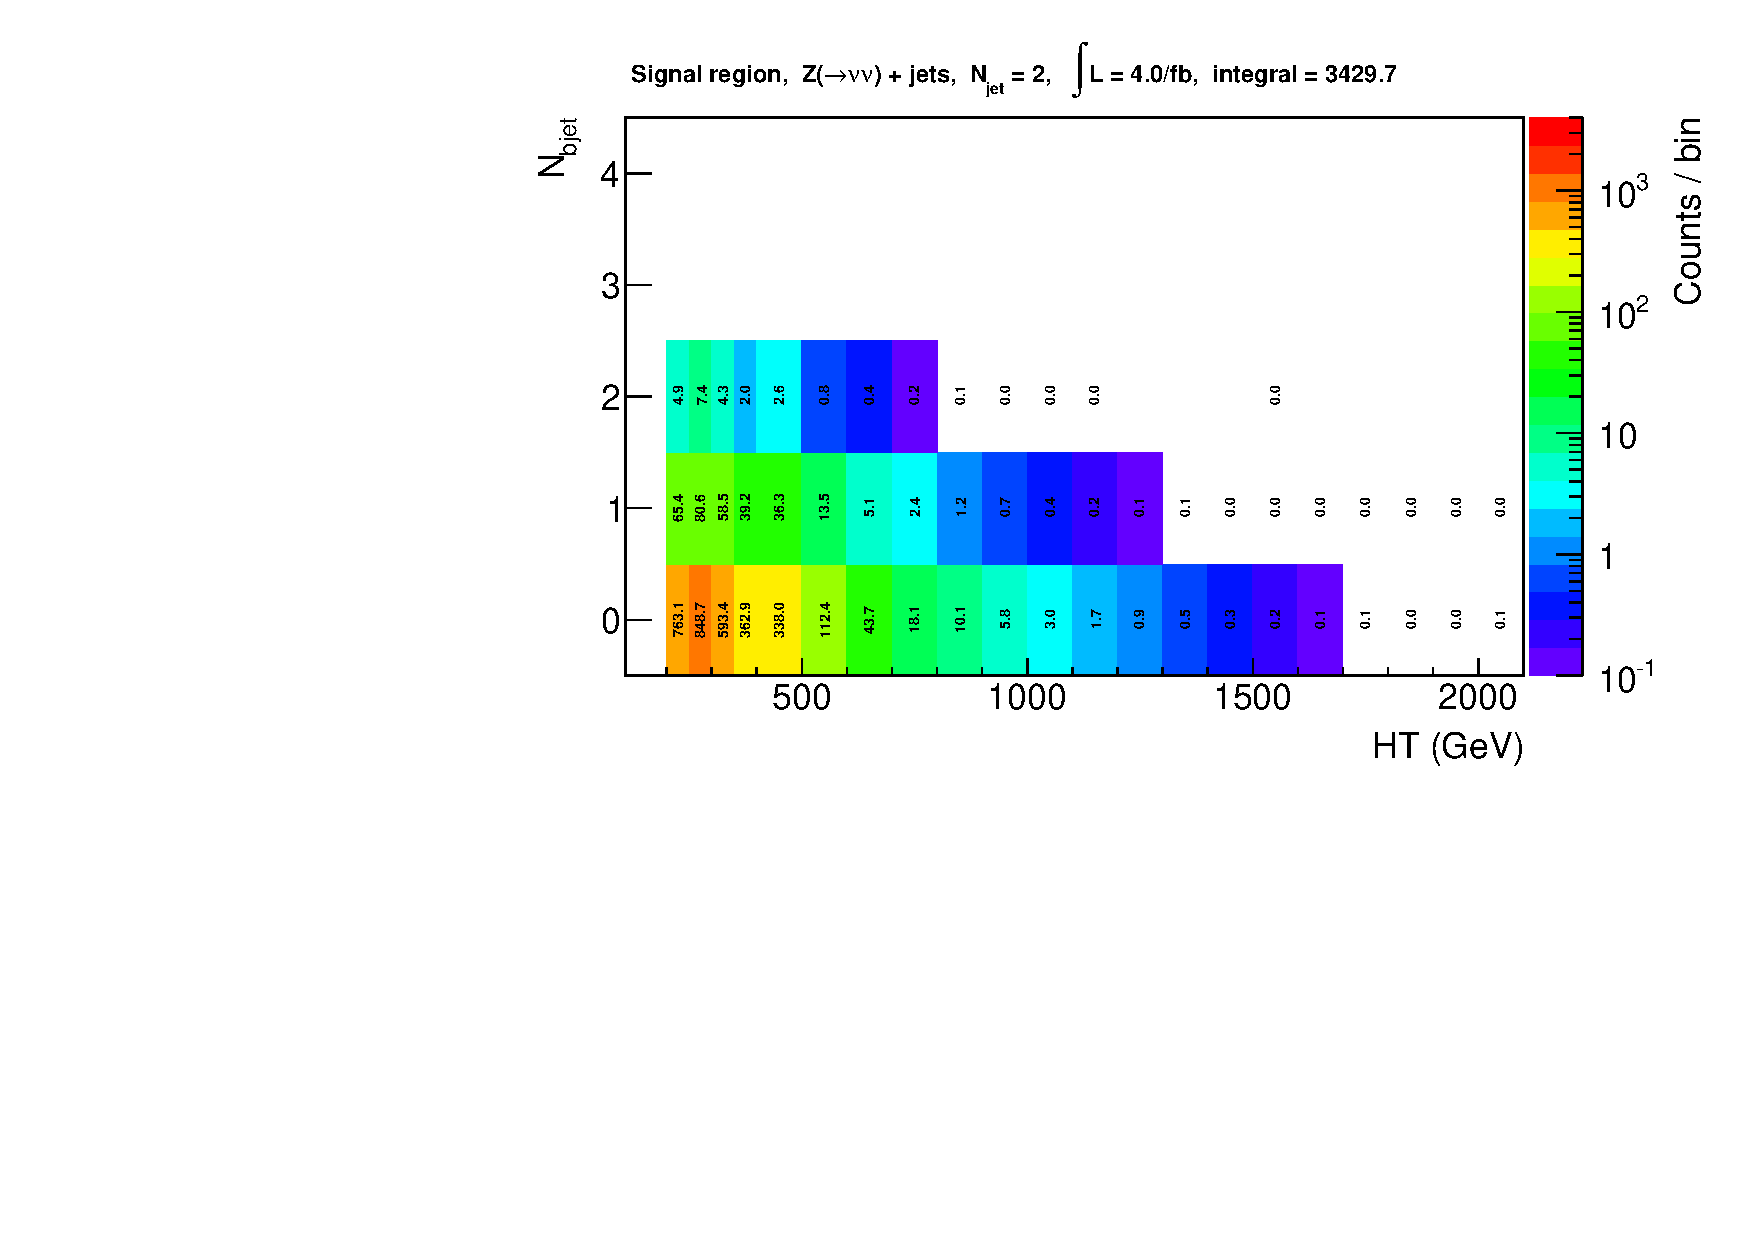
\includegraphics[width=0.5\textwidth]{figures/yieldPlots/had_zinv_eq2j.pdf}
  }\\
  \subfigure[Hadronic signal region yields for W~+~jets backtround
  ($\njet = 2$)]{
    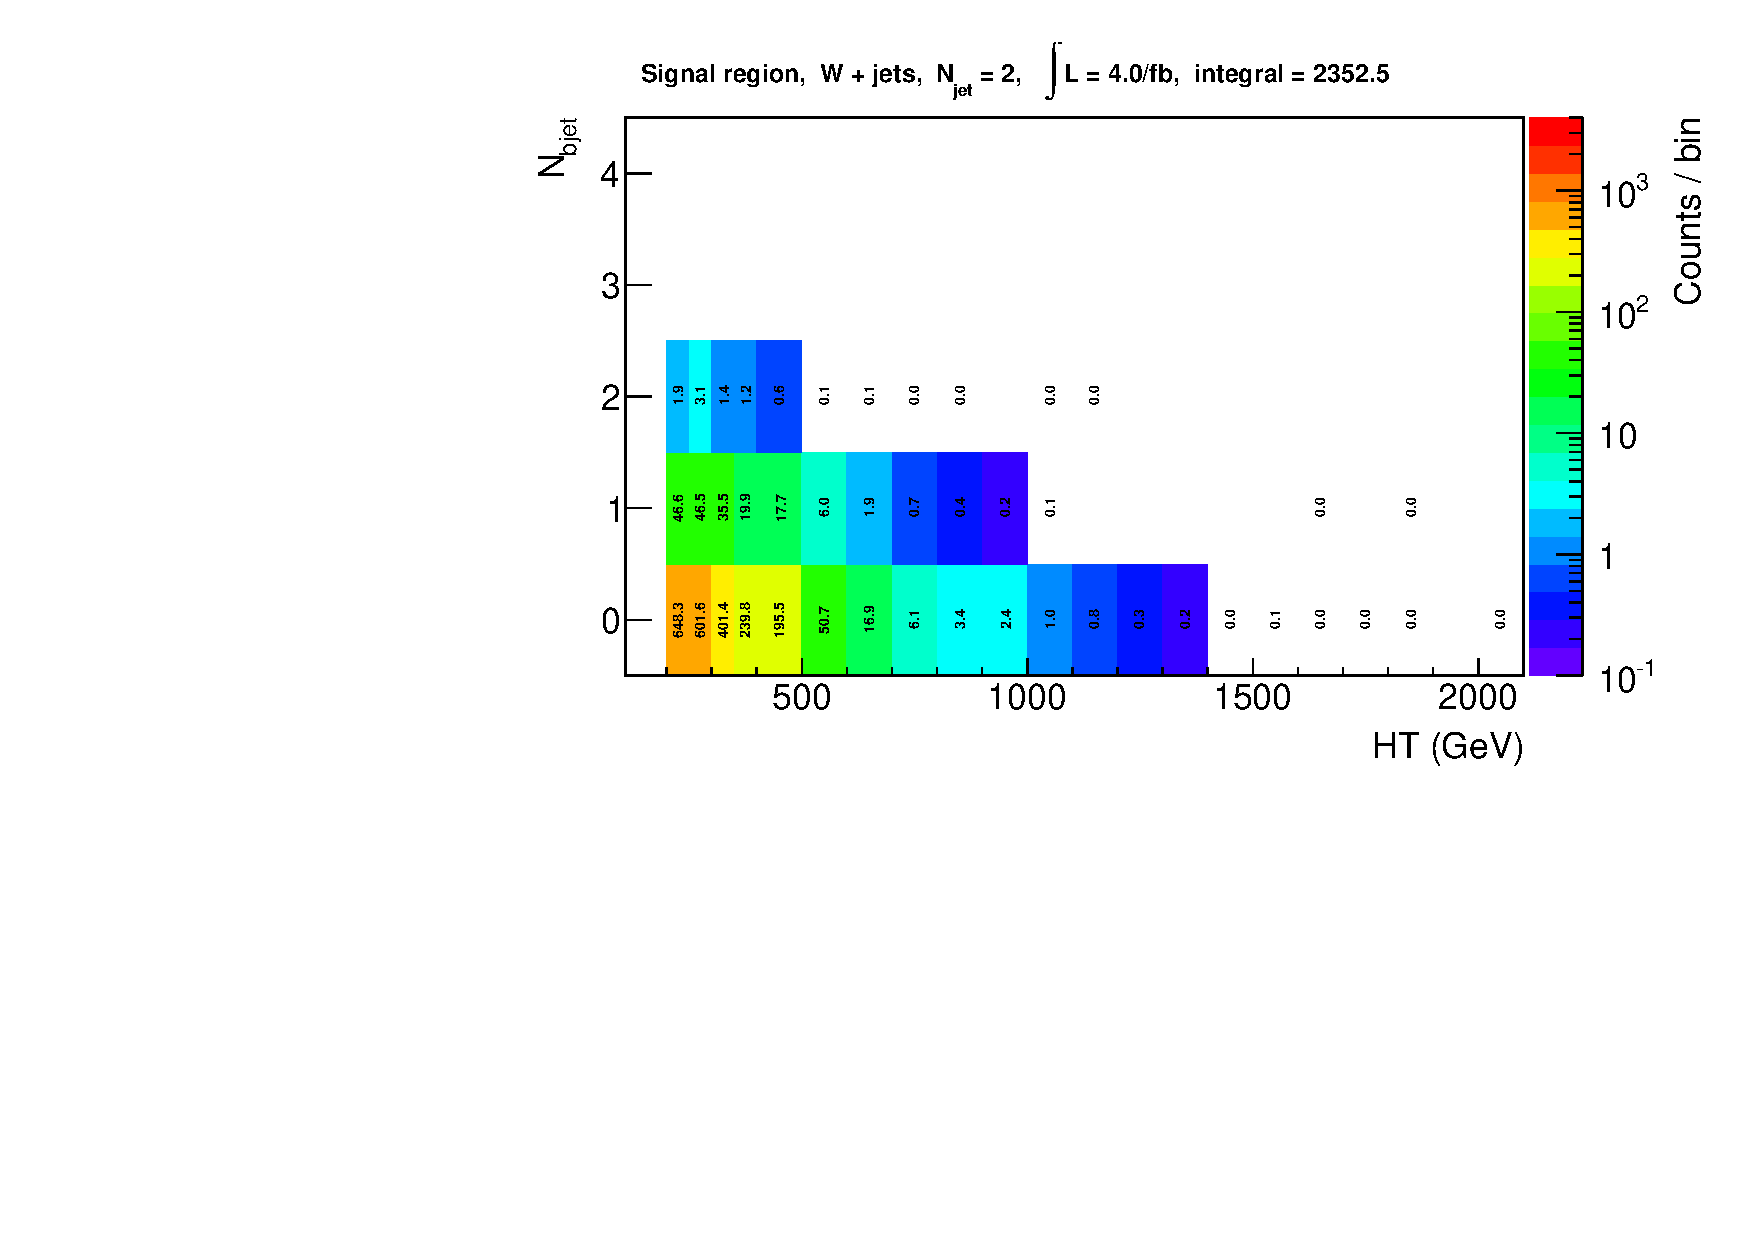
\includegraphics[width=0.5\textwidth]{figures/yieldPlots/had_wjets_eq2j.pdf}
  }~~
  \subfigure[Hadronic signal region yields for \ttbar background
  ($\njet = 2$)]{
    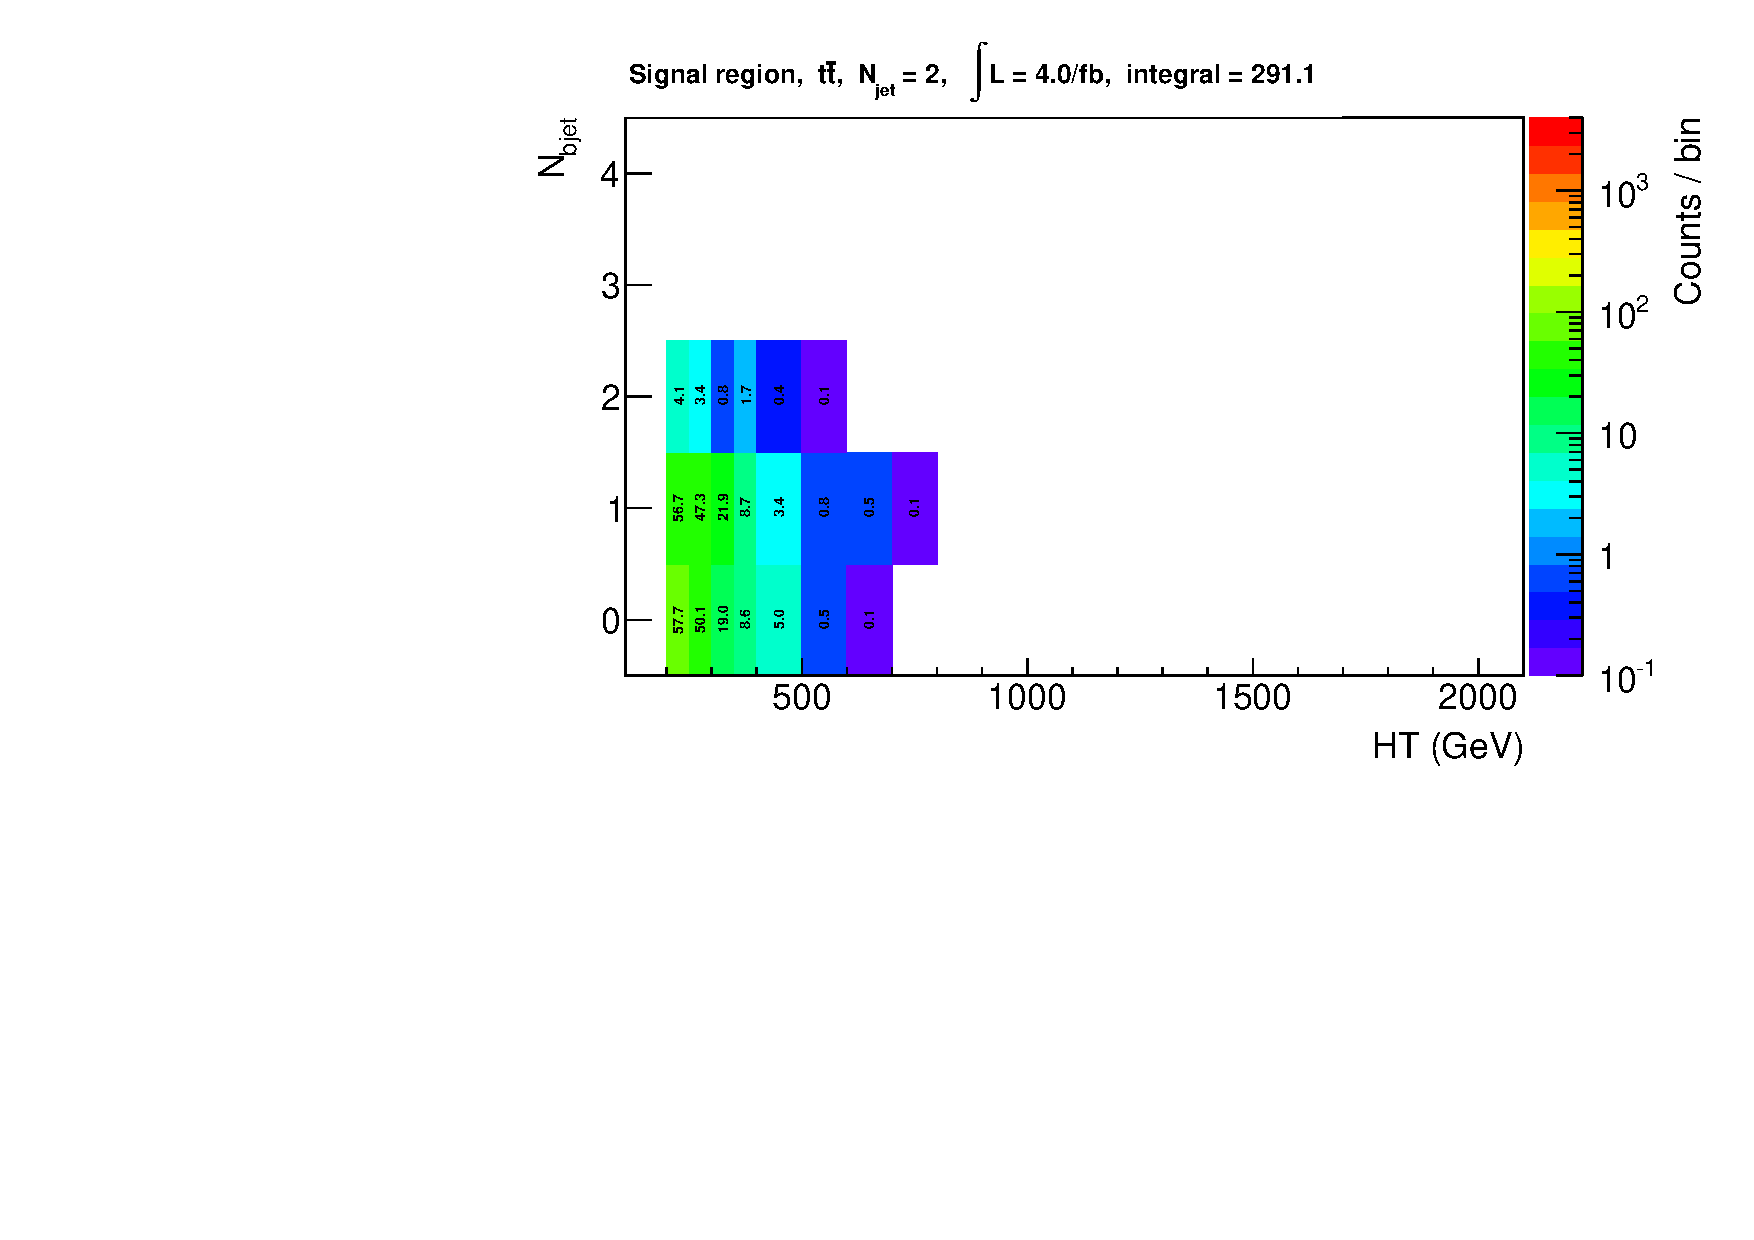
\includegraphics[width=0.5\textwidth]{figures/yieldPlots/had_ttbar_eq2j.pdf}
  }
  \\
  \subfigure[Hadronic signal region yields for electroweak backgrounds
  ($\njet = 3$)]{
    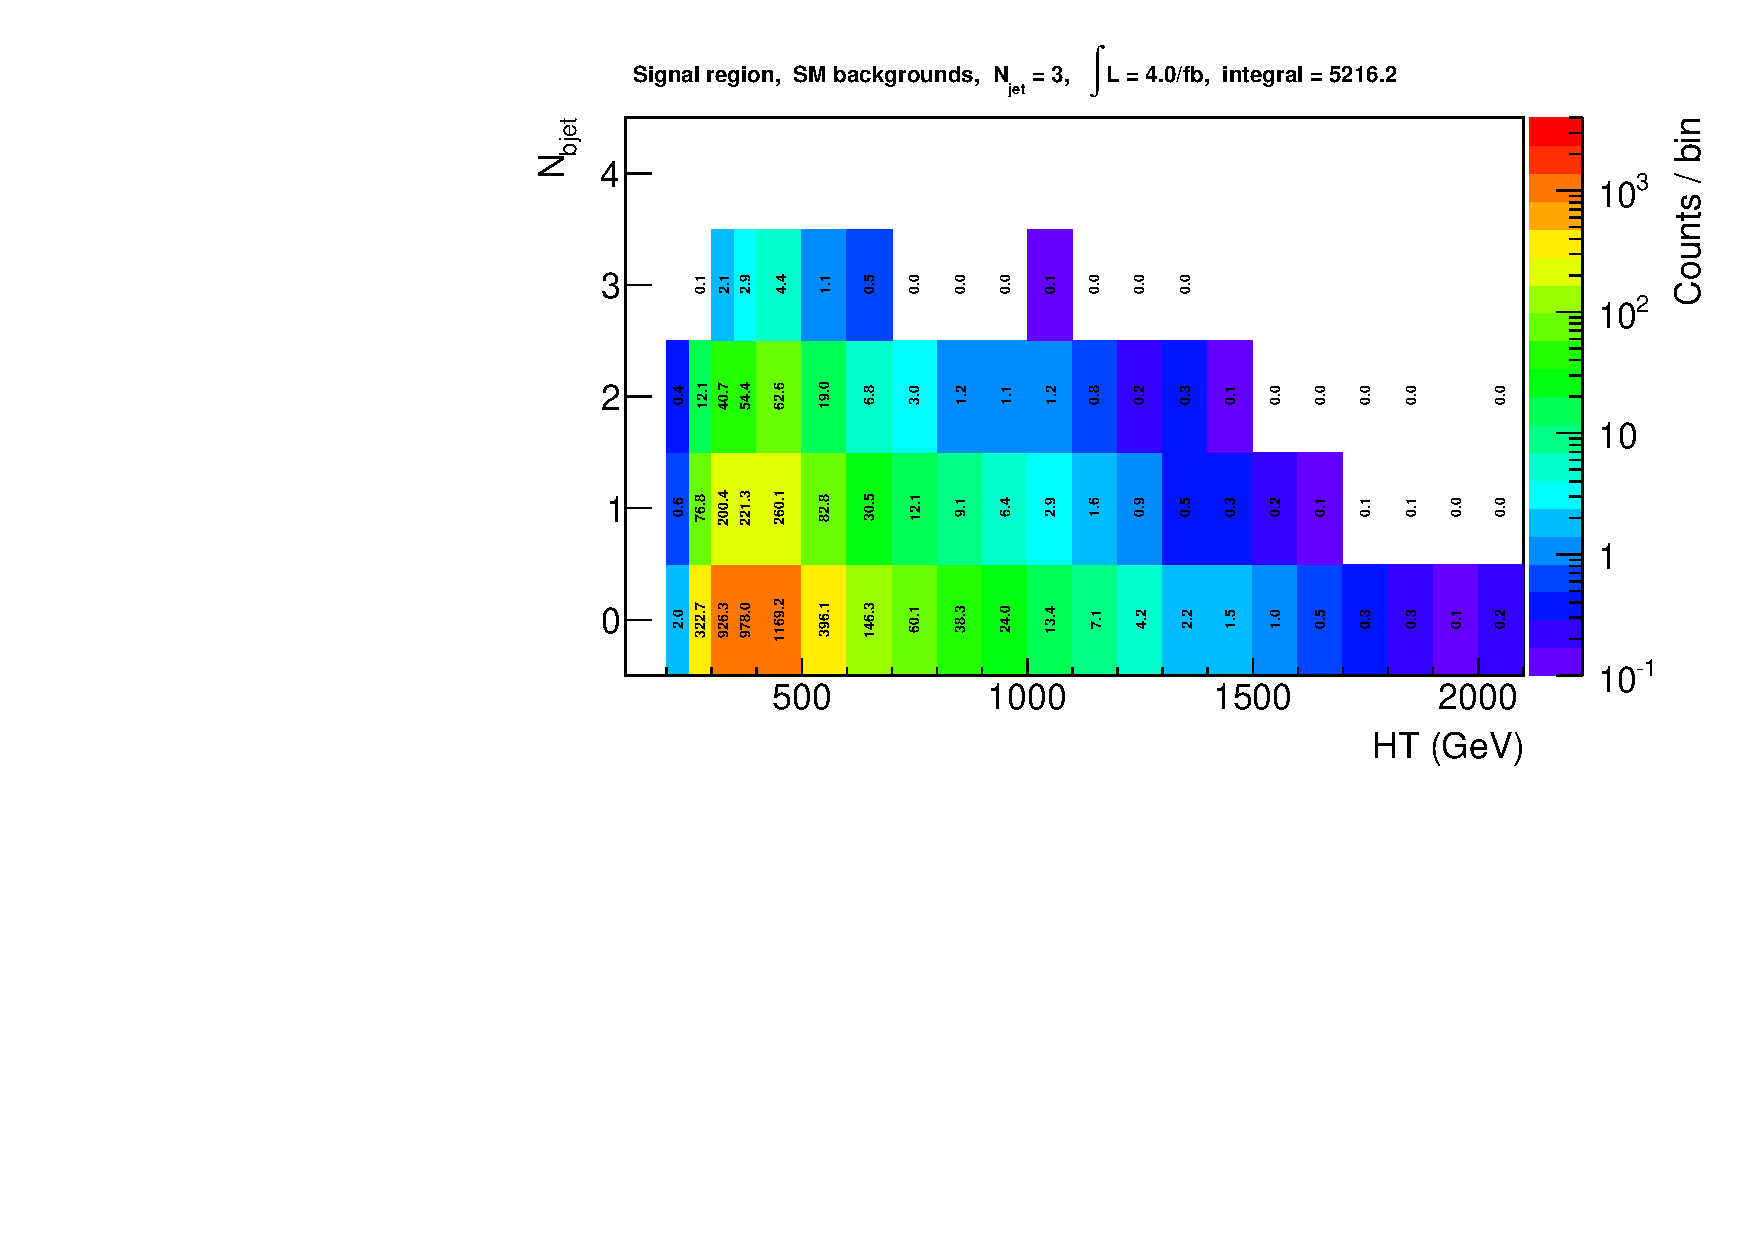
\includegraphics[width=0.5\textwidth]{figures/yieldPlots/had_ewk_eq3j.pdf}
  }~~
  \subfigure[Hadronic signal region yields for the \zinv background
  ($\njet = 3$)]{
    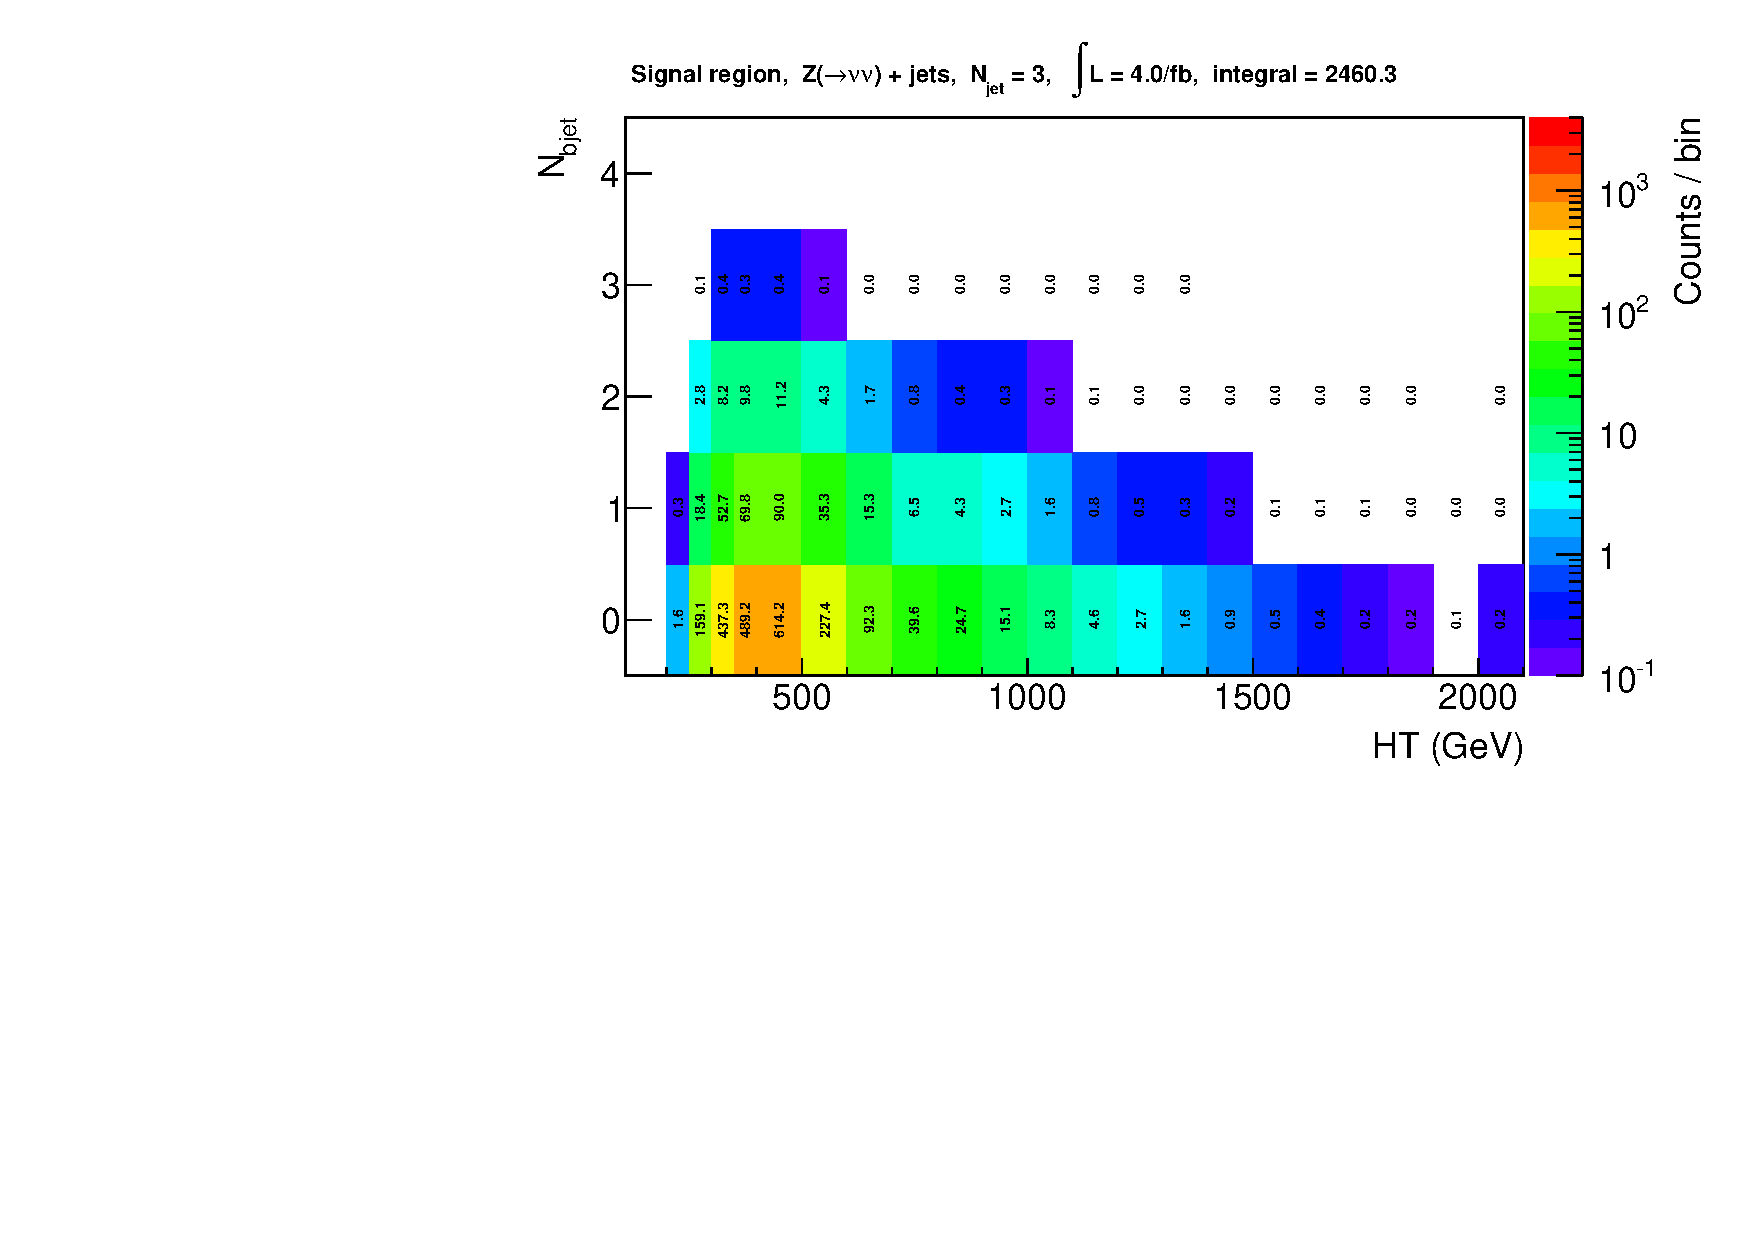
\includegraphics[width=0.5\textwidth]{figures/yieldPlots/had_zinv_eq3j.pdf}
  }\\
  \subfigure[Hadronic signal region yields for W~+~jets backtround
  ($\njet = 3$)]{
    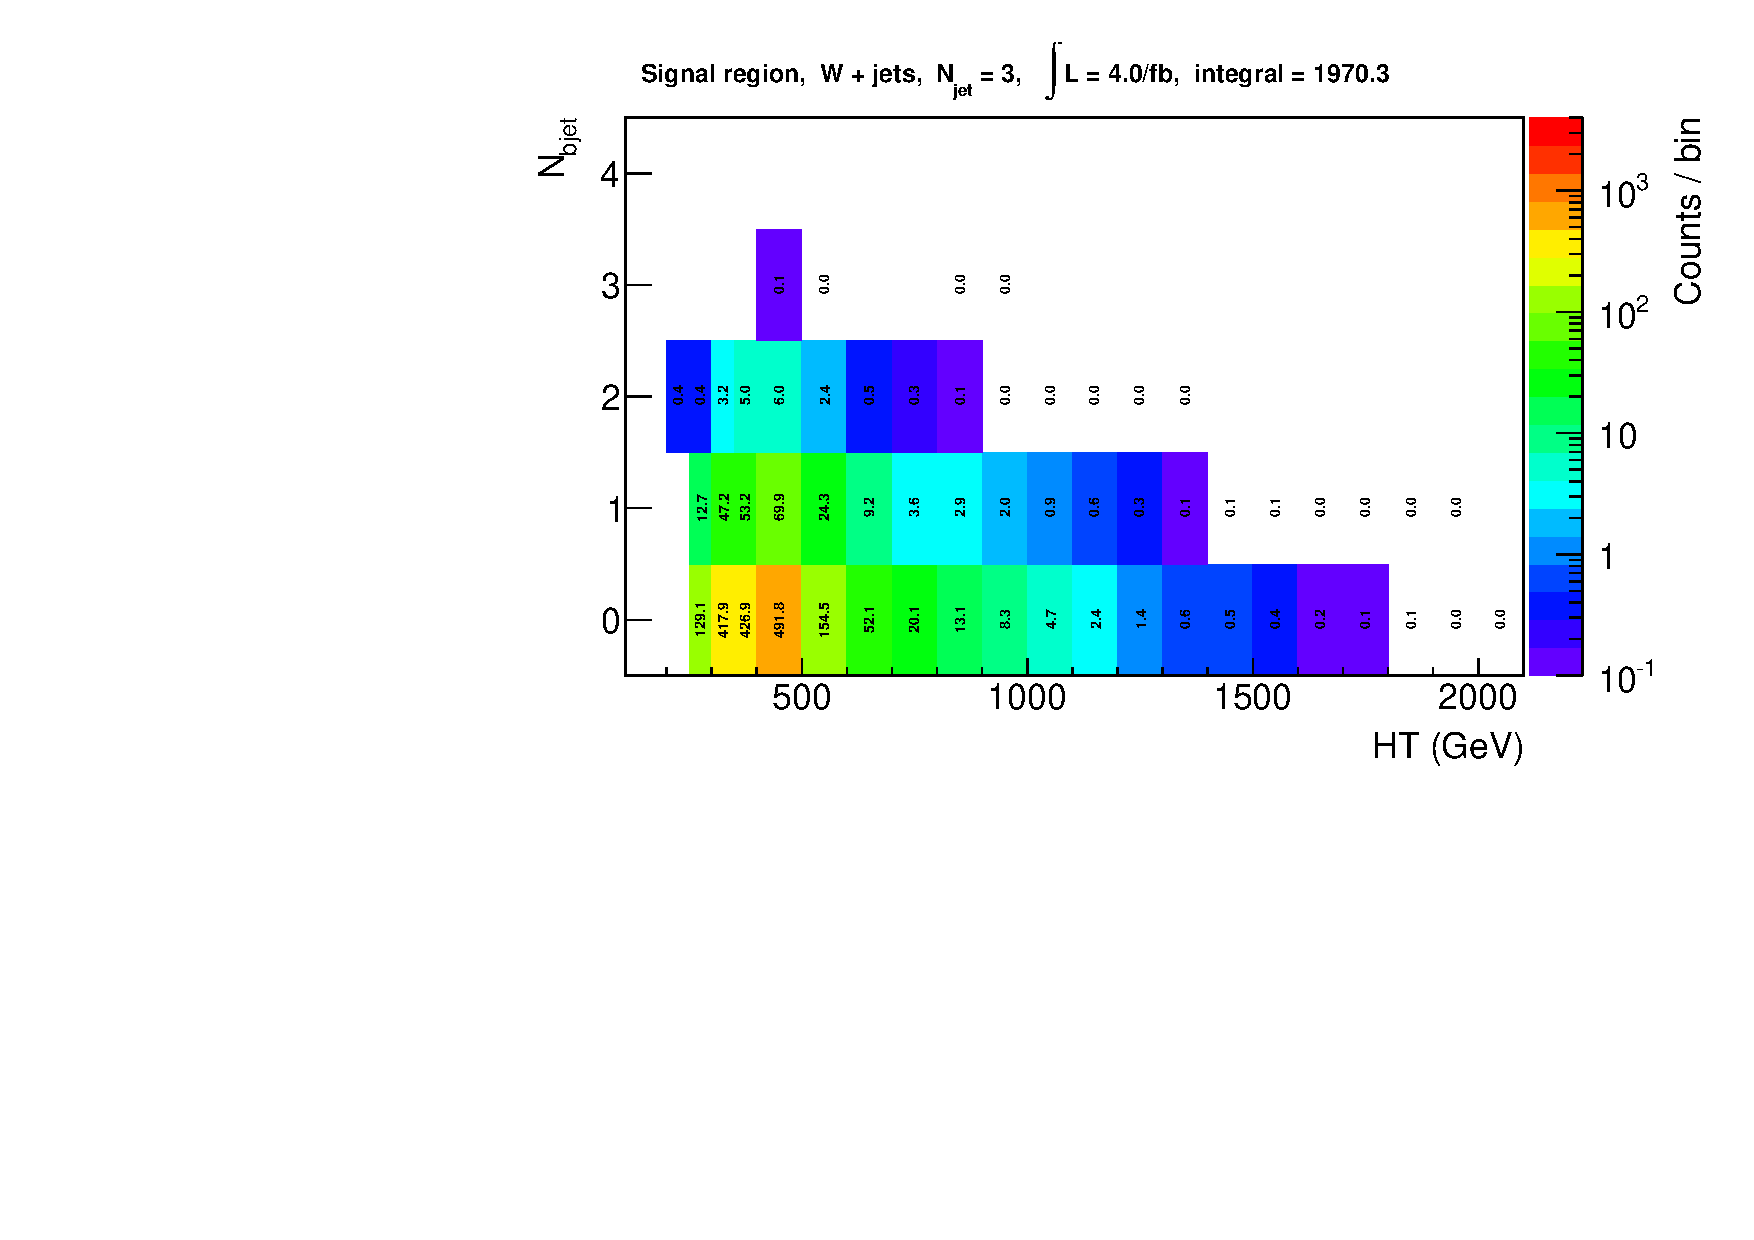
\includegraphics[width=0.5\textwidth]{figures/yieldPlots/had_wjets_eq3j.pdf}
  }~~
  \subfigure[Hadronic signal region yields for \ttbar background
  ($\njet = 3$)]{
    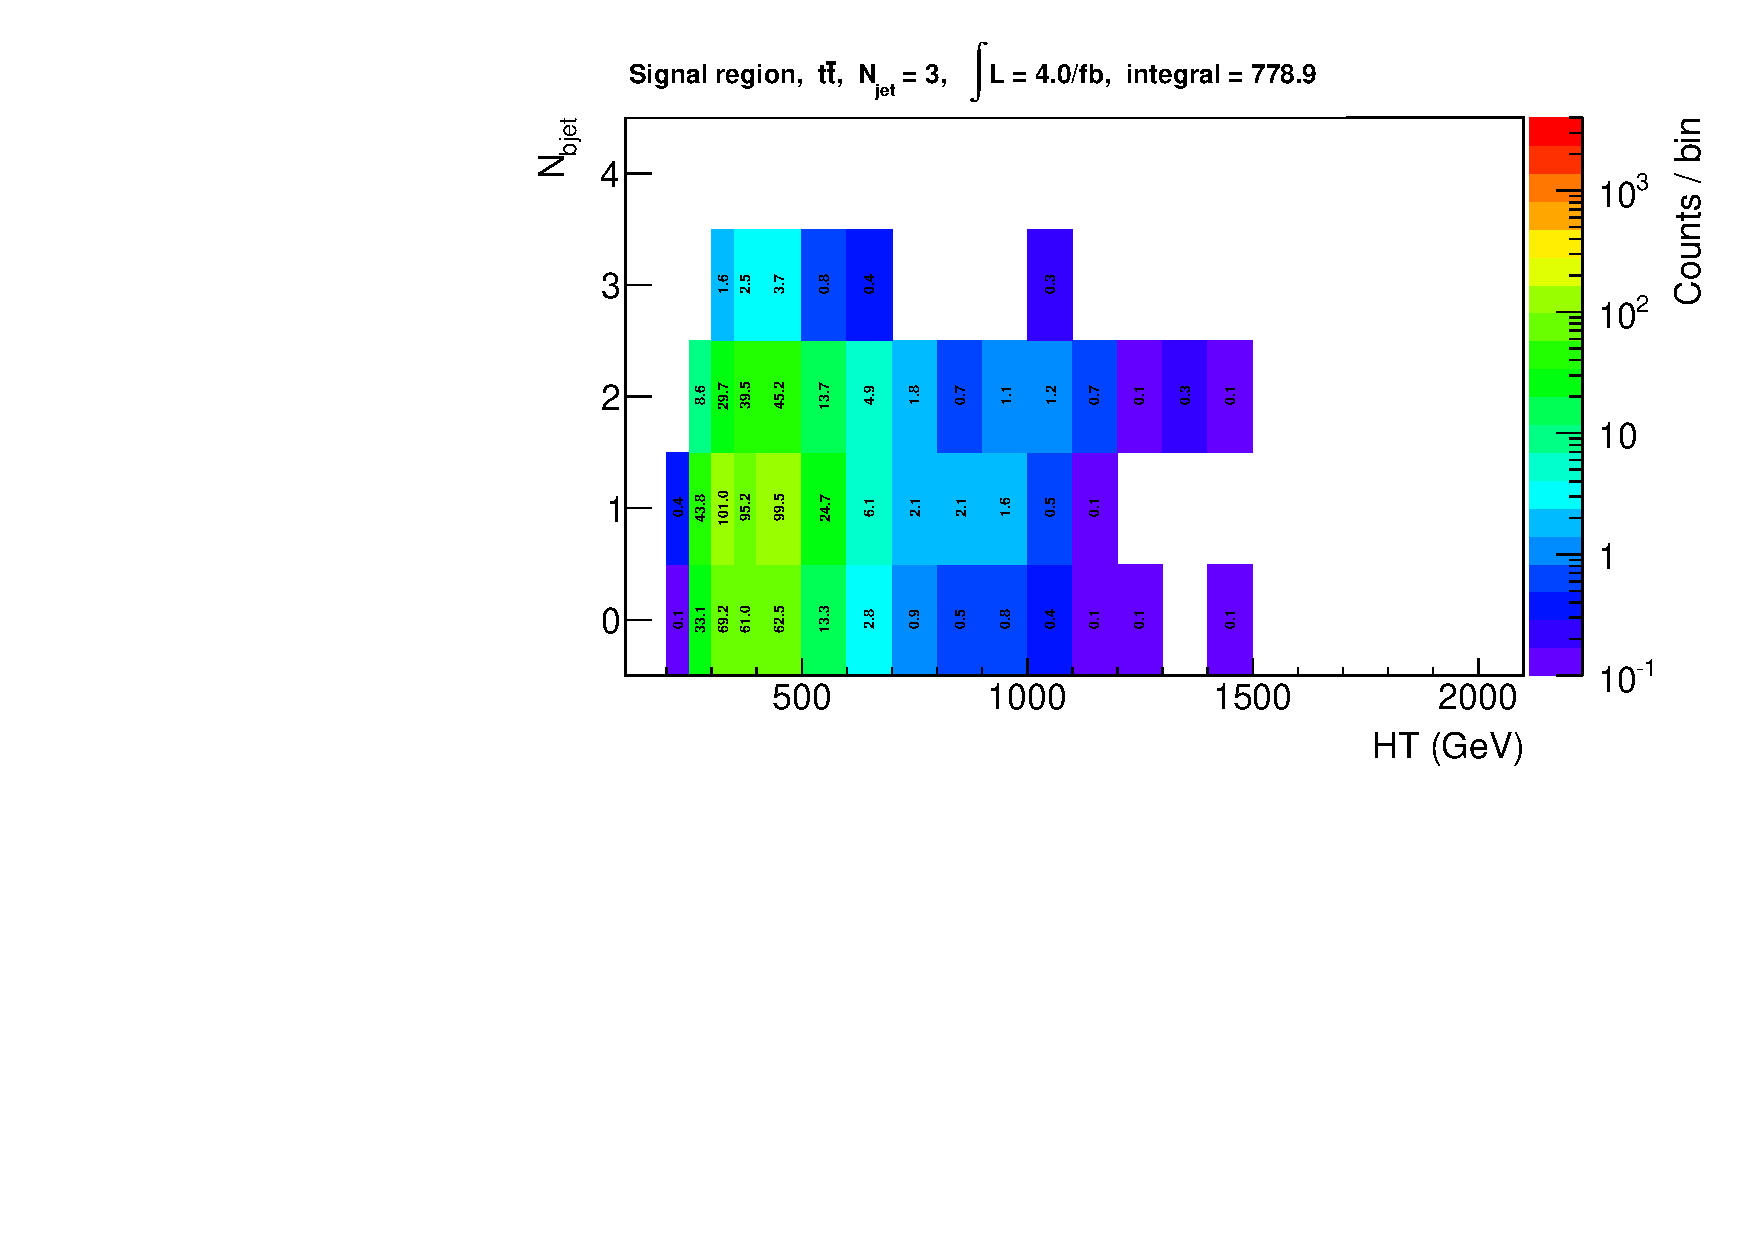
\includegraphics[width=0.5\textwidth]{figures/yieldPlots/had_ttbar_eq3j.pdf}
  }

  \\
  \subfigure[Hadronic signal region yields for electroweak backgrounds
  ($\njet = 4$)]{
    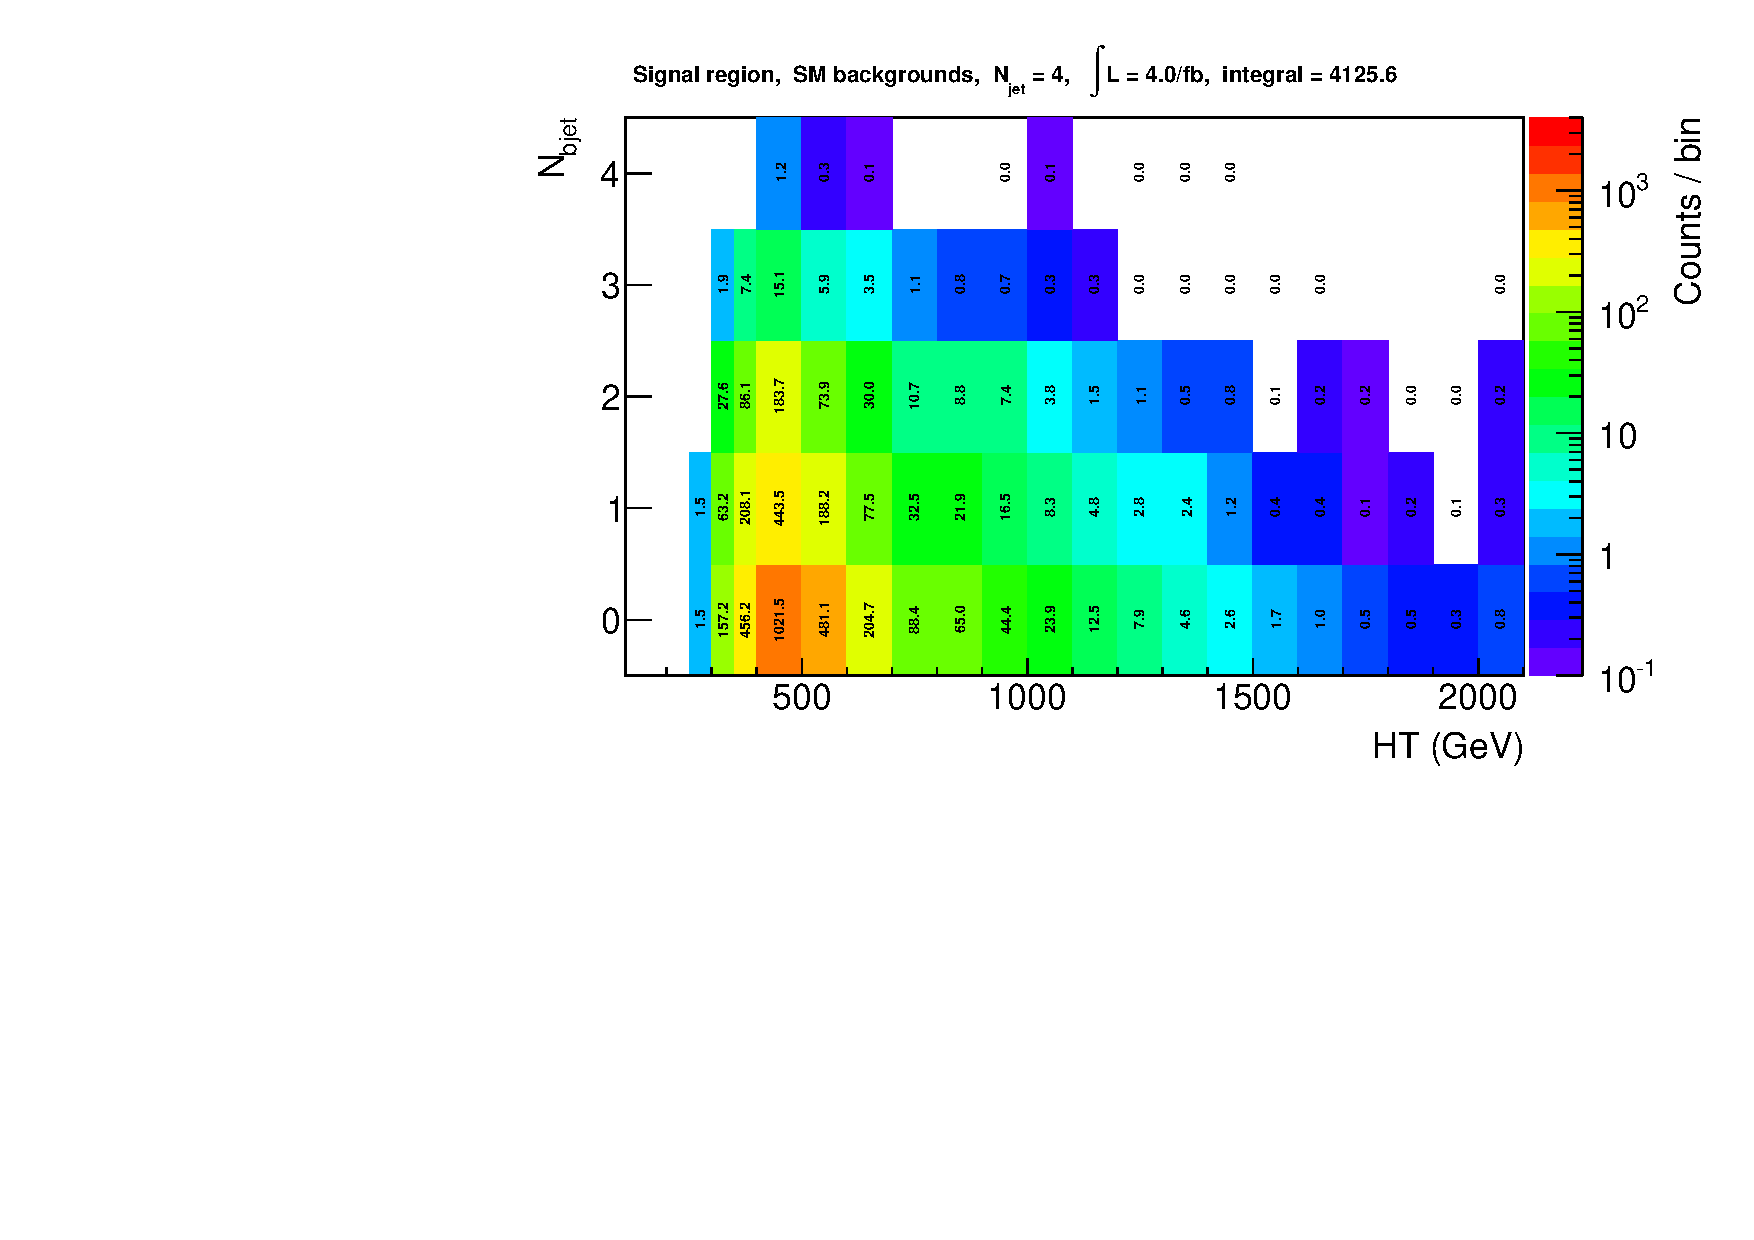
\includegraphics[width=0.5\textwidth]{figures/yieldPlots/had_ewk_eq4j.pdf}
  }~~
  \subfigure[Hadronic signal region yields for the \zinv background
  ($\njet = 4$)]{
    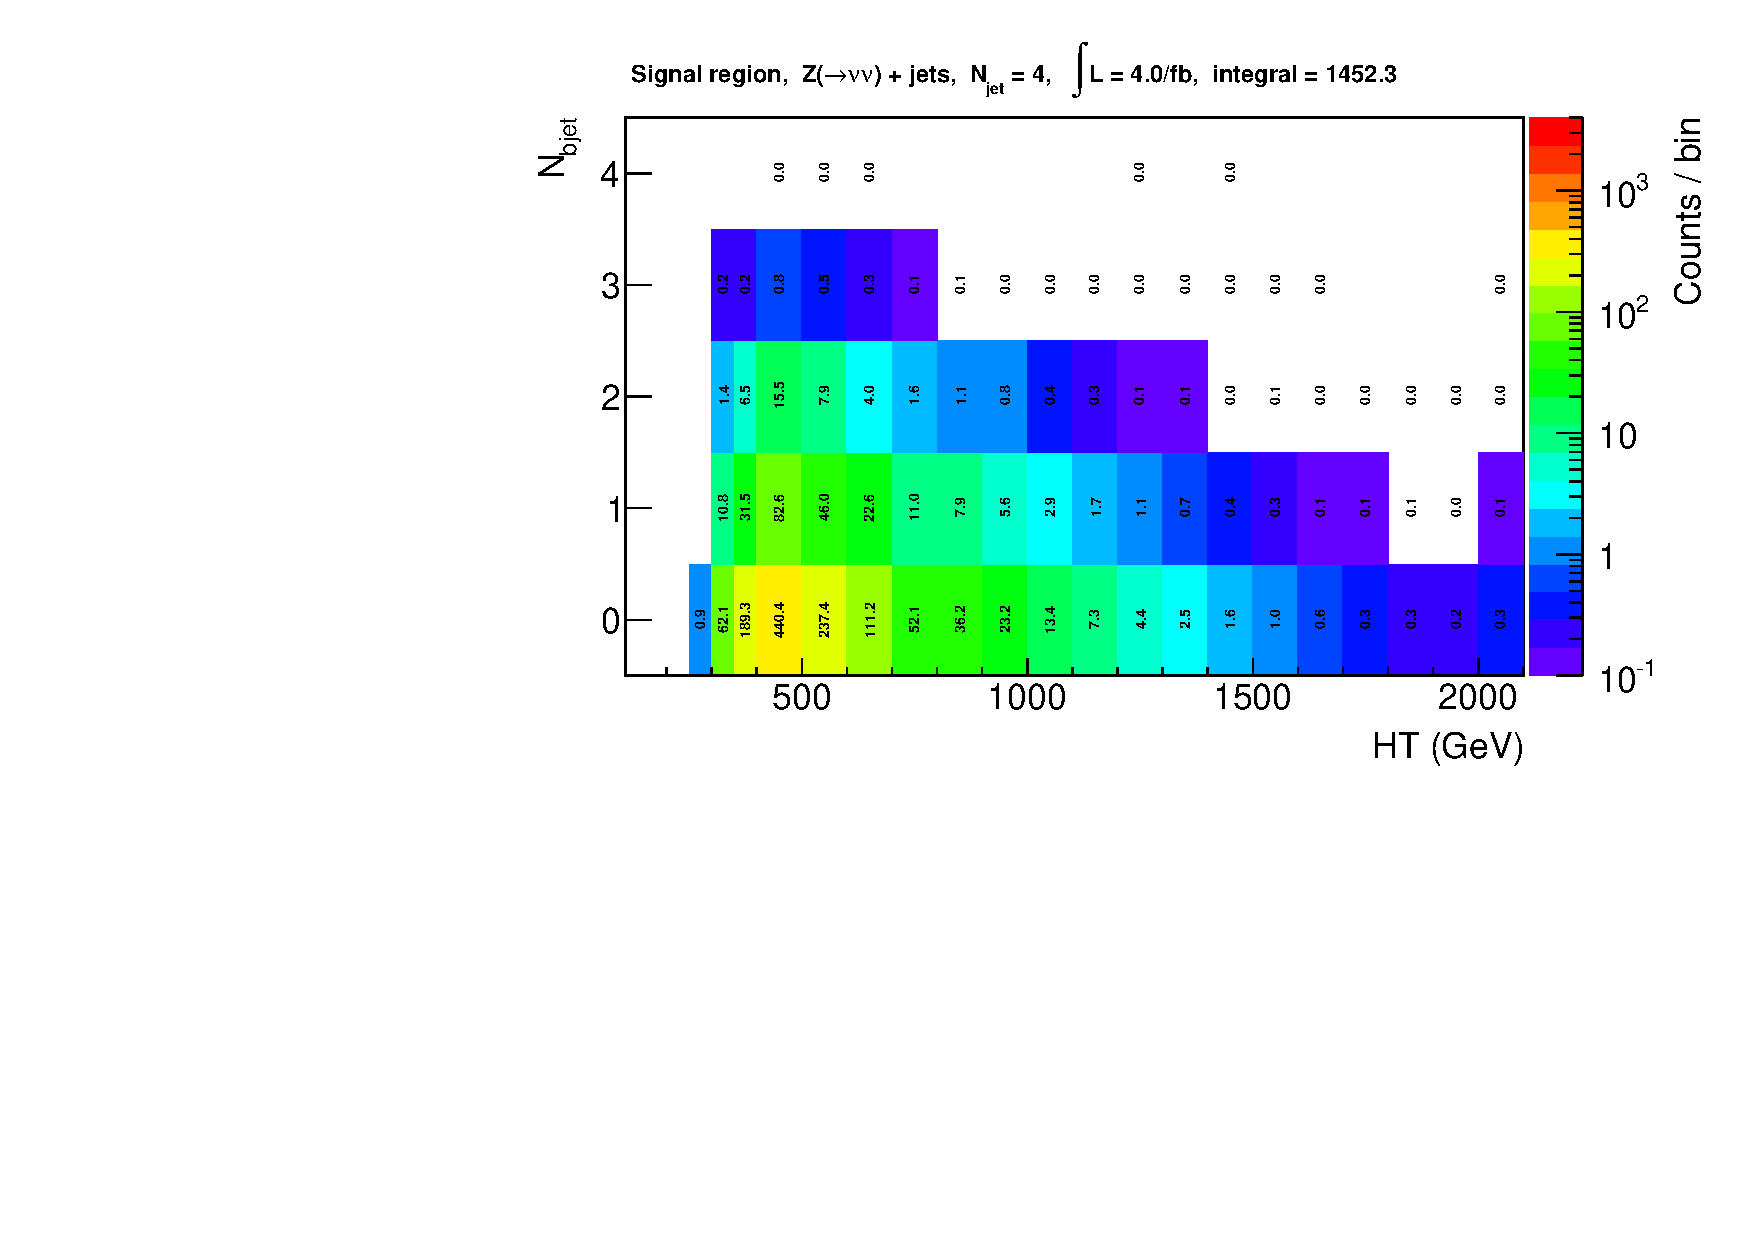
\includegraphics[width=0.5\textwidth]{figures/yieldPlots/had_zinv_eq4j.pdf}
  }\\
  \subfigure[Hadronic signal region yields for W~+~jets backtround
  ($\njet = 4$)]{
    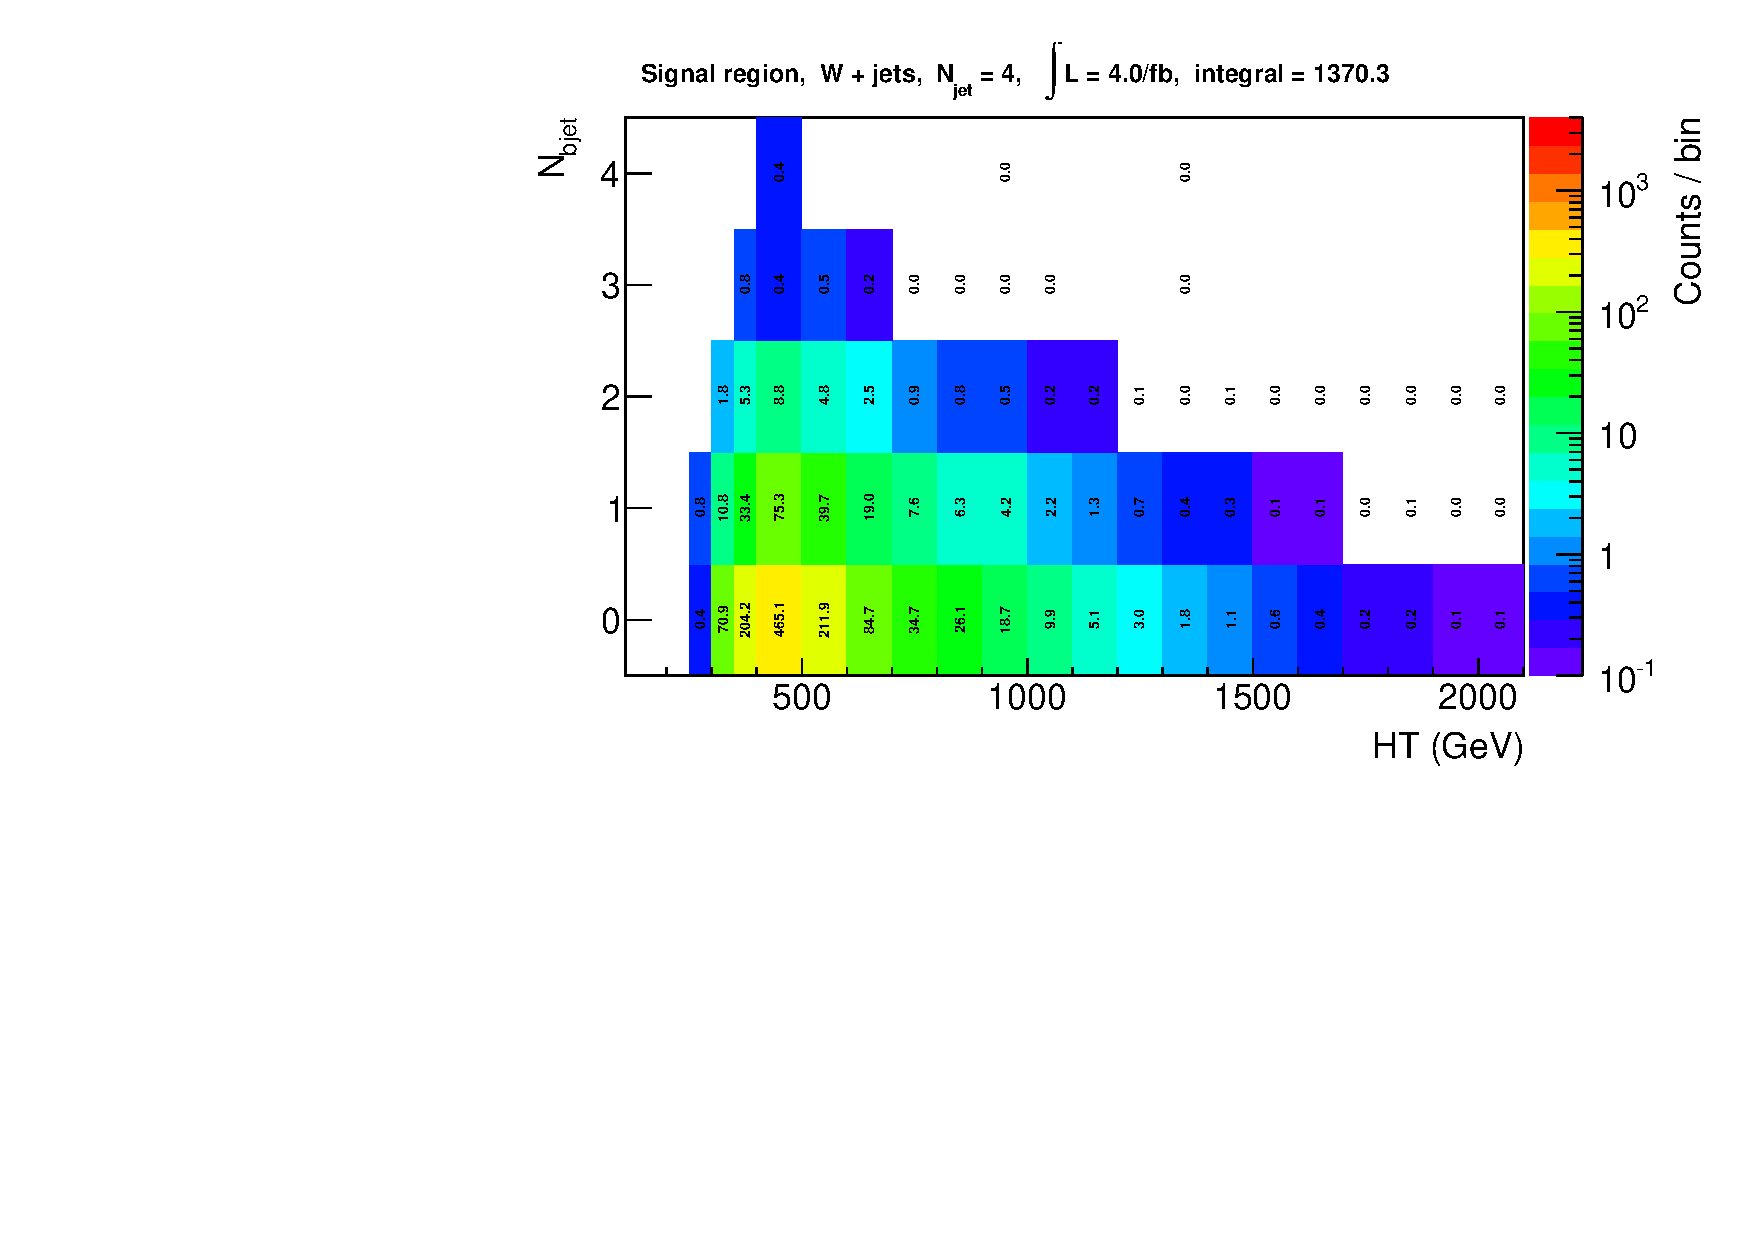
\includegraphics[width=0.5\textwidth]{figures/yieldPlots/had_wjets_eq4j.pdf}
  }~~
  \subfigure[Hadronic signal region yields for \ttbar background
  ($\njet = 4$)]{
    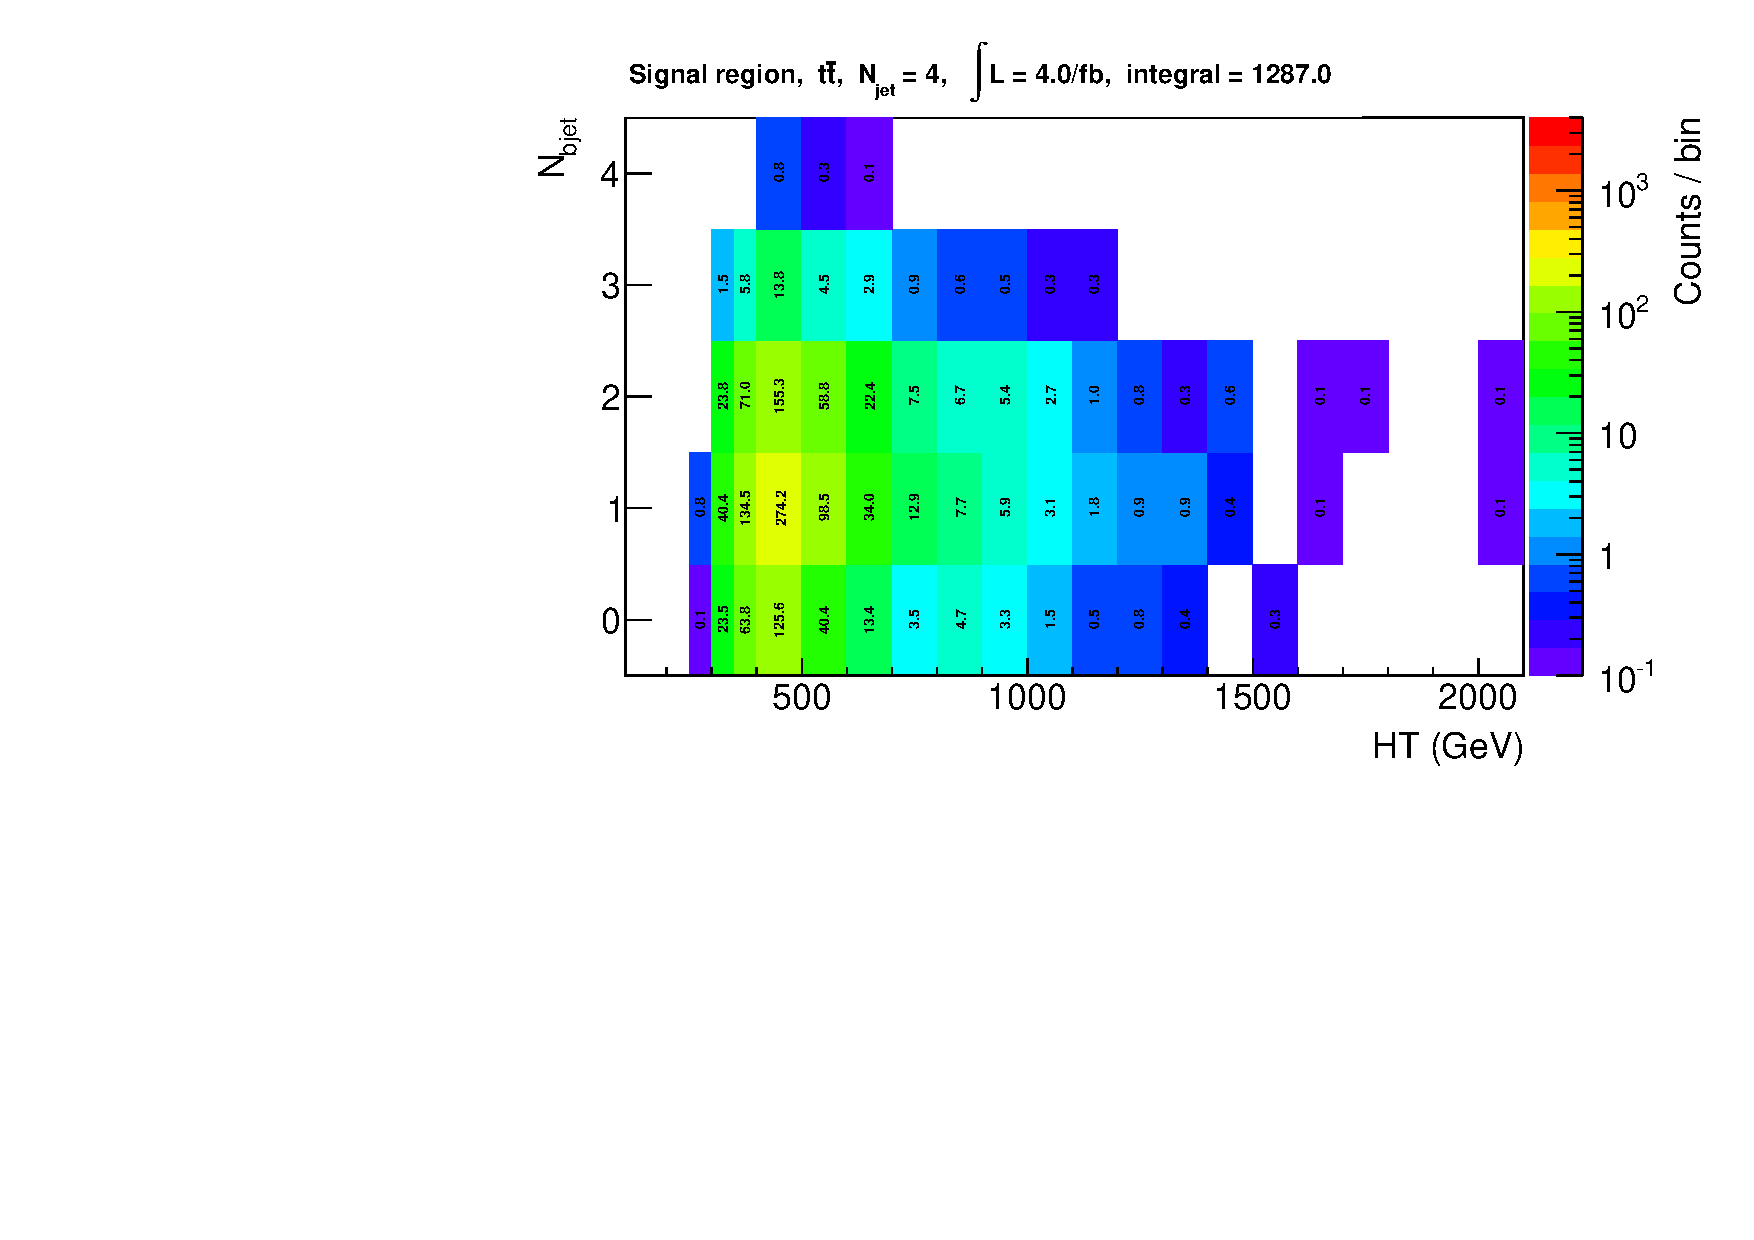
\includegraphics[width=0.5\textwidth]{figures/yieldPlots/had_ttbar_eq4j.pdf}
  }

  \\
  \subfigure[Hadronic signal region yields for electroweak backgrounds
  ($\njet \geq 5$)]{
    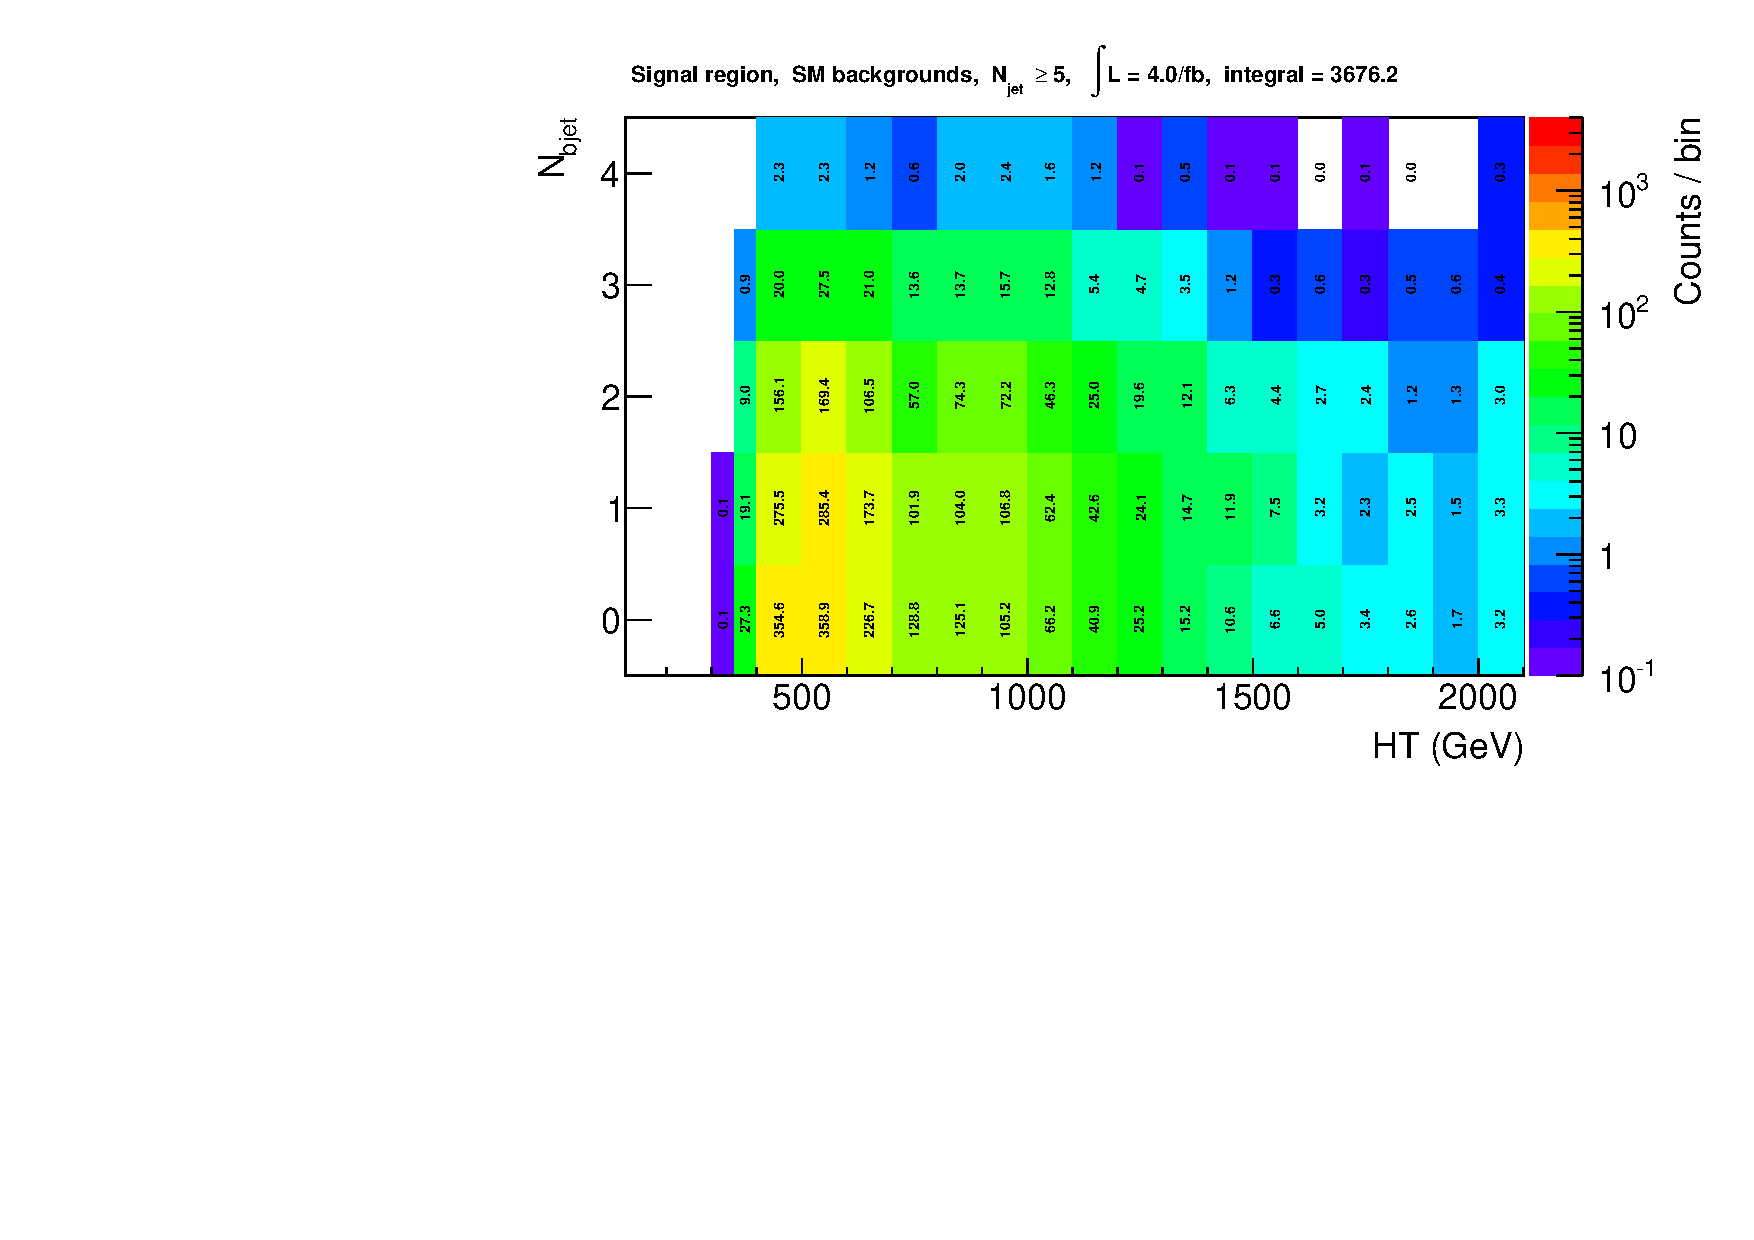
\includegraphics[width=0.5\textwidth]{figures/yieldPlots/had_ewk_ge5j.pdf}
  } ~~
  \subfigure[Hadronic signal region yields for the \zinv background
  ($\njet \geq 5$)]{
    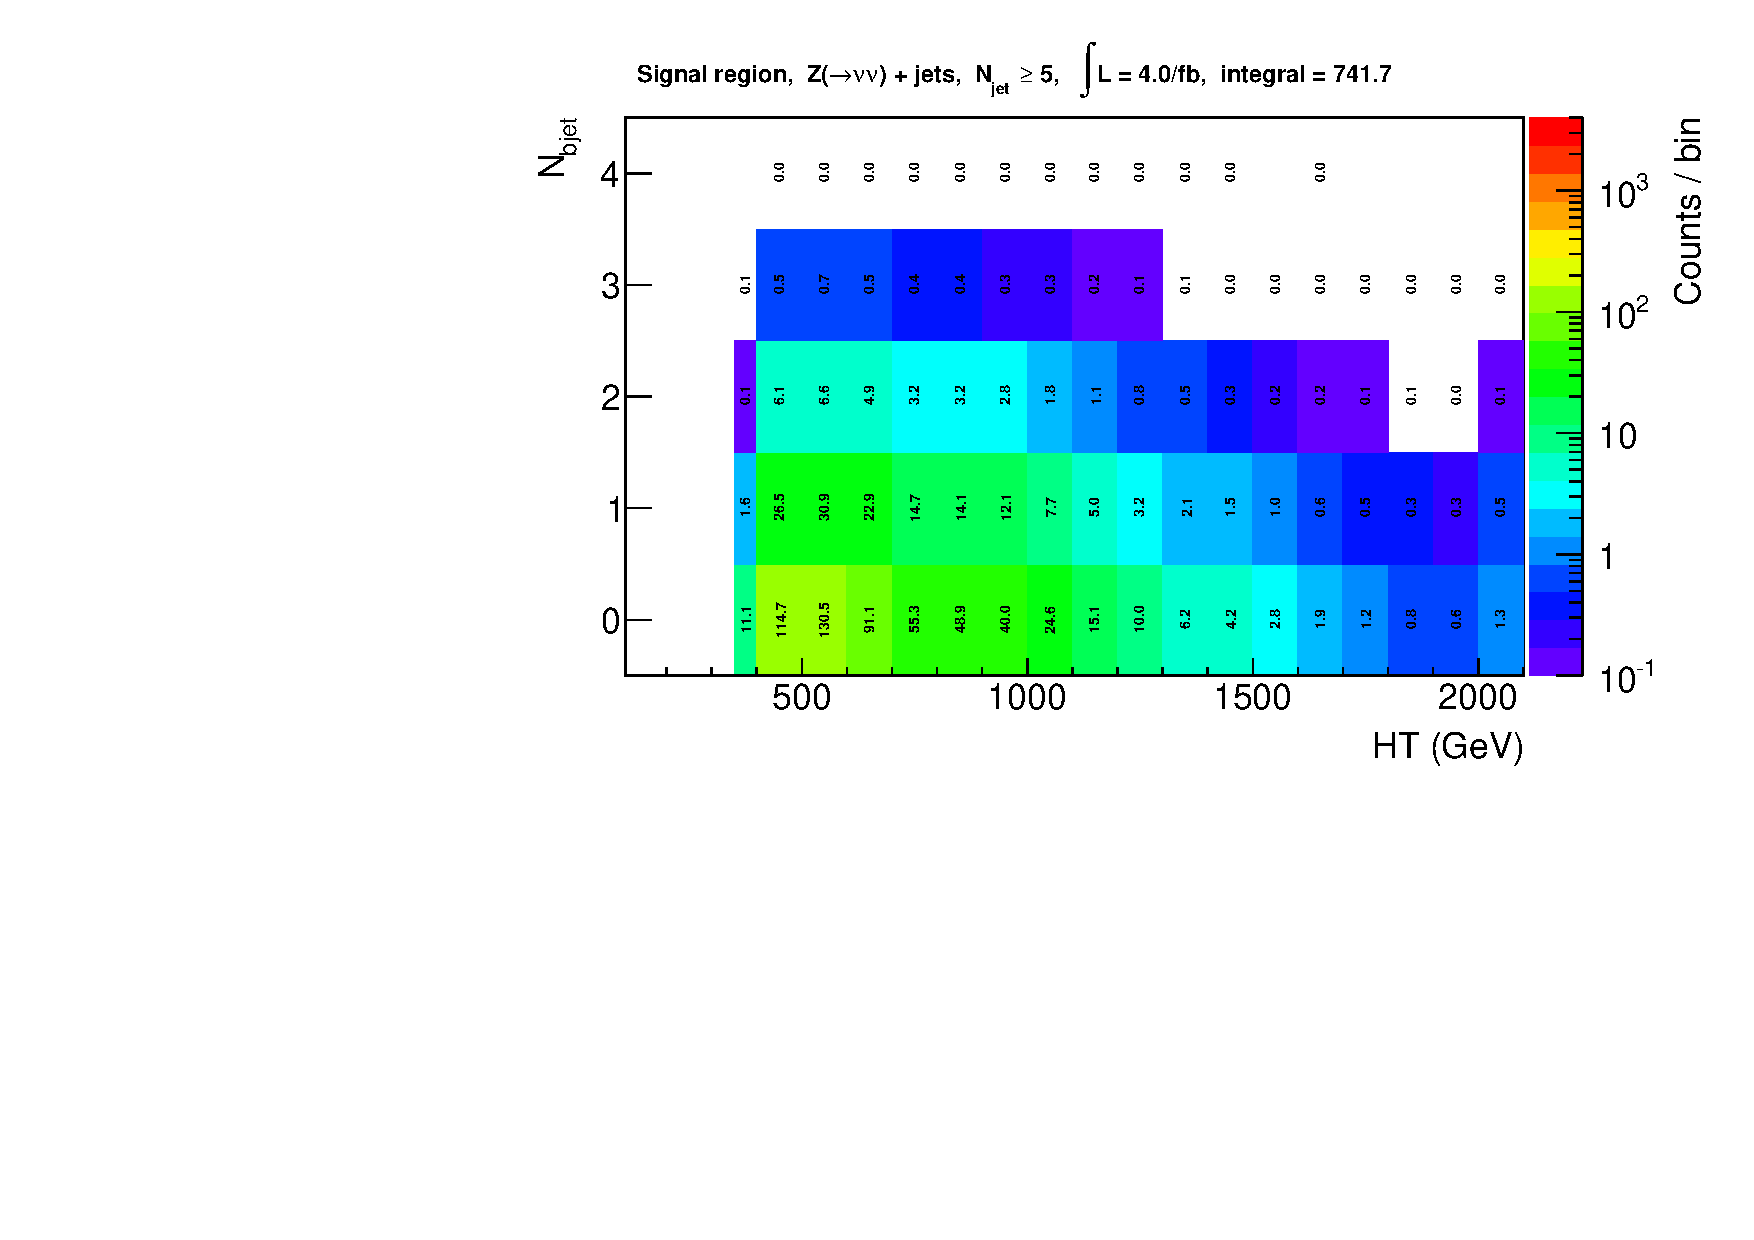
\includegraphics[width=0.5\textwidth]{figures/yieldPlots/had_zinv_ge5j.pdf}
  }\\
  \subfigure[Hadronic signal region yields for W~+~jets backtround
  ($\njet \geq 5$)]{
    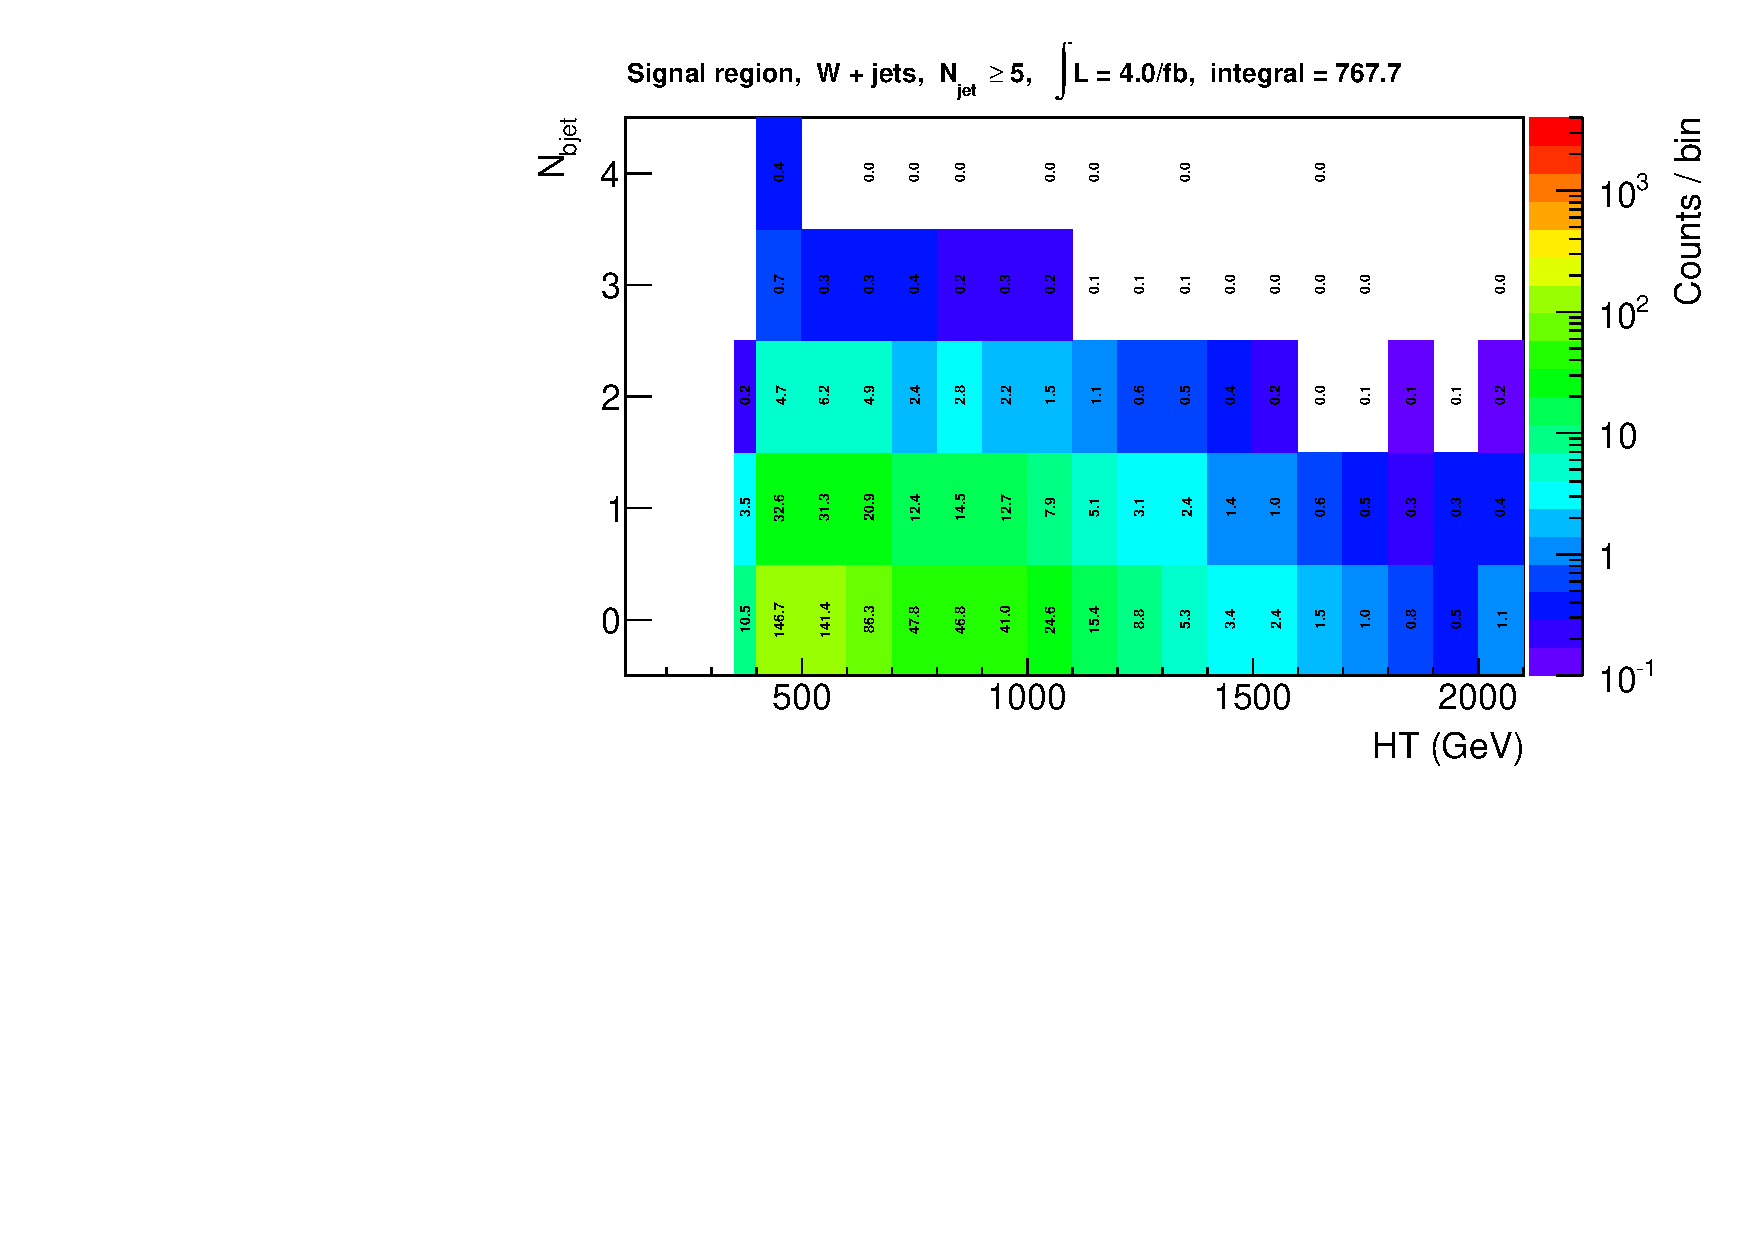
\includegraphics[width=0.5\textwidth]{figures/yieldPlots/had_wjets_ge5j.pdf}
  }~~
  \subfigure[Hadronic signal region yields for \ttbar background
  ($\njet \geq 5$)]{
    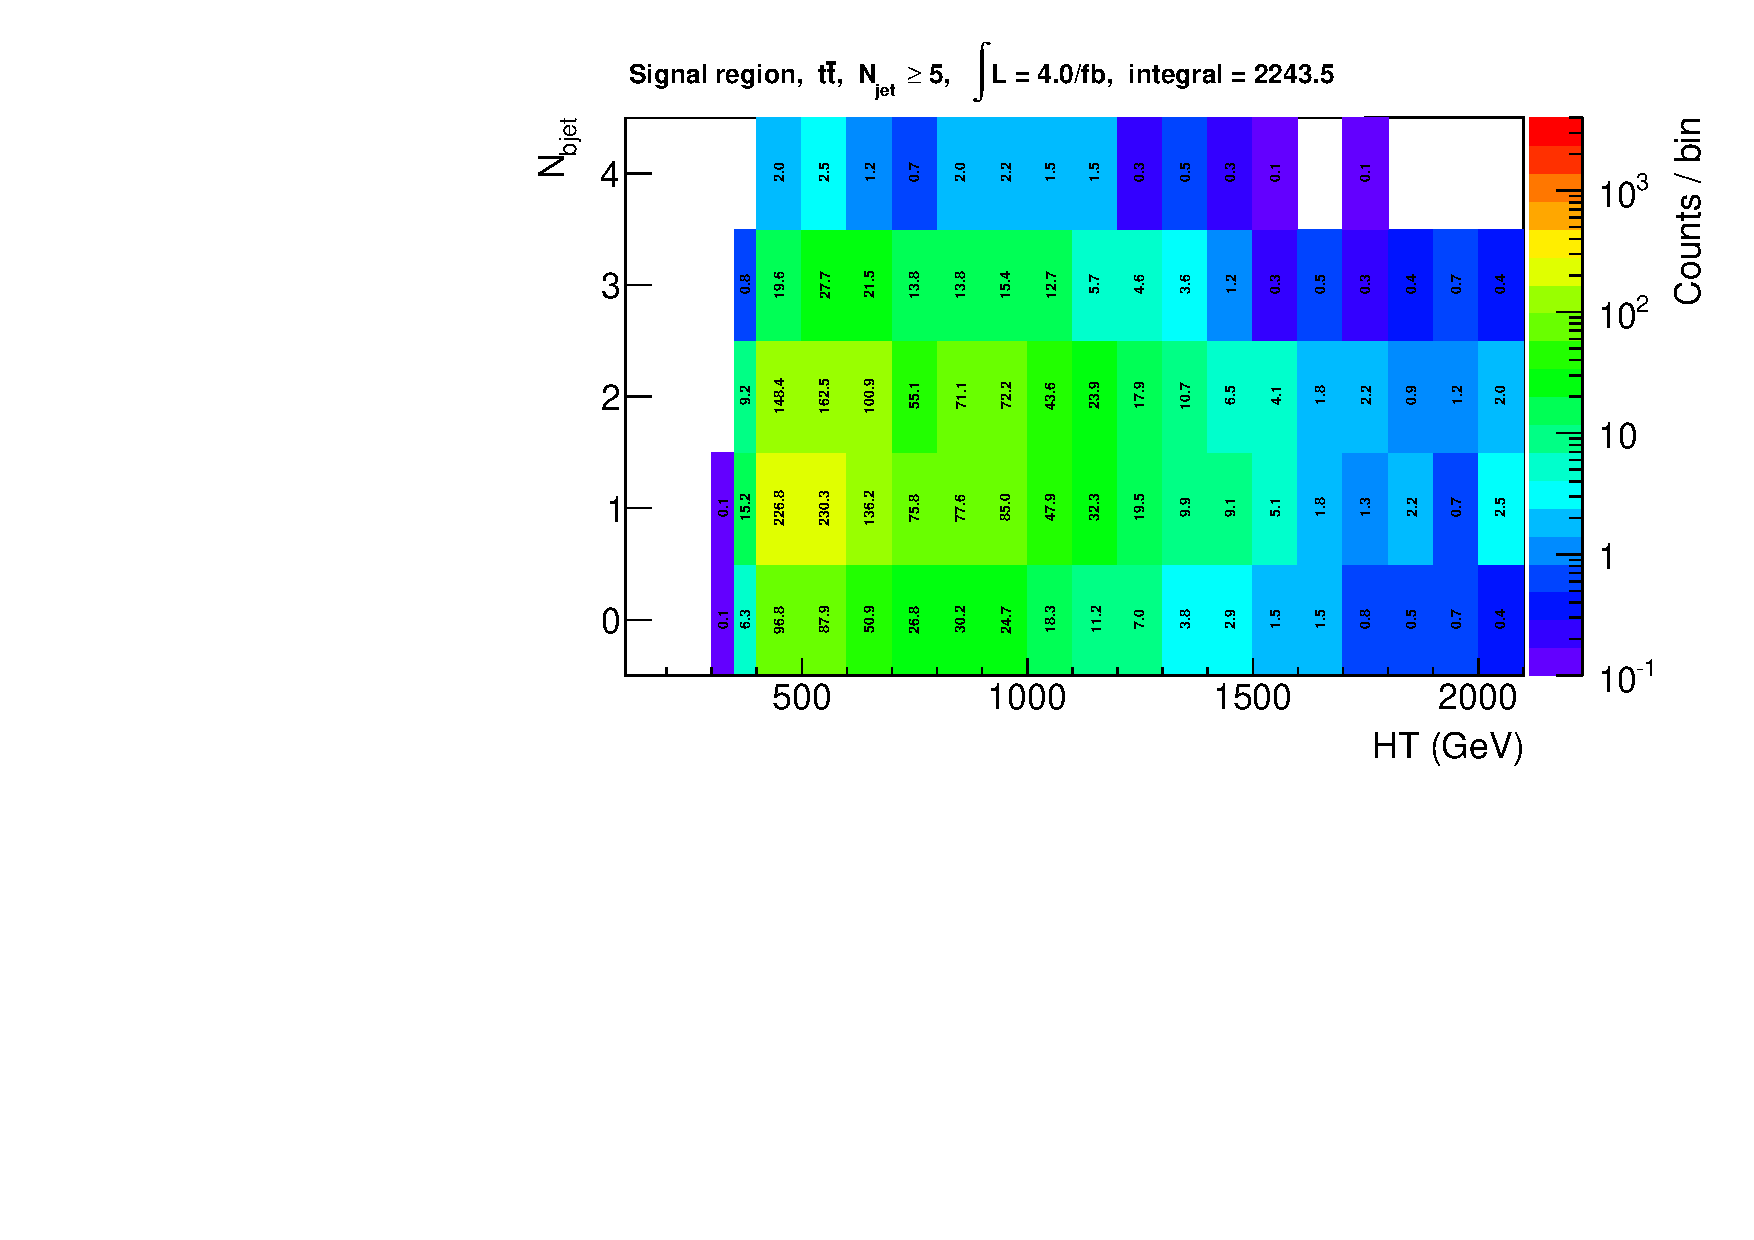
\includegraphics[width=0.5\textwidth]{figures/yieldPlots/had_ttbar_ge5j.pdf}
  }

  \\
  \subfigure[Hadronic signal region yields for T1bbbb simplified model 
  ($\njet \geq 5$)]{
    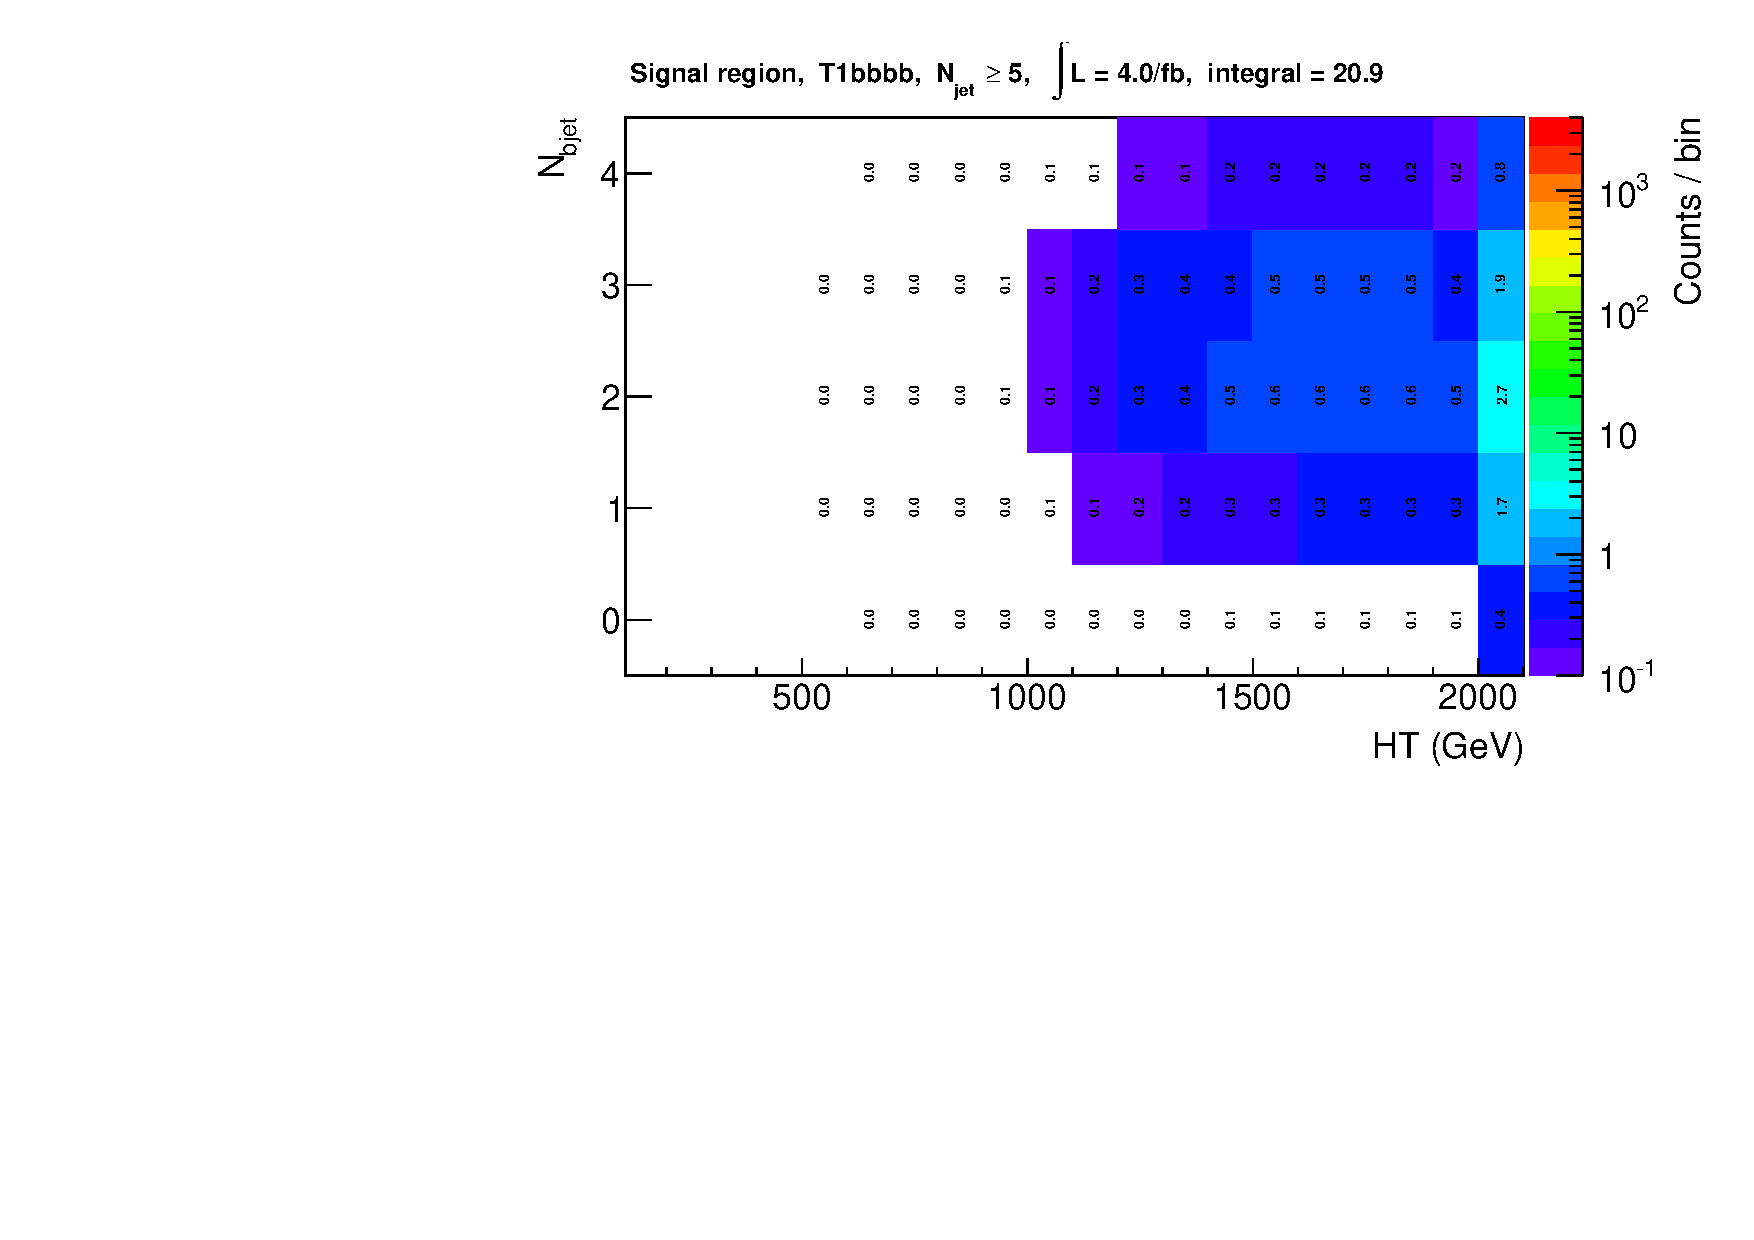
\includegraphics[width=0.5\textwidth]{figures/yieldPlots/sig_T1bbbb_ge5j.pdf}
  }
  \\
  \caption{\label{fig:ewkYields} Yields at $4\fbinv$ for the electroweak backgrounds in the
  hadronic signal region. Split up with the analysis bins. }
\end{figure}

%%____________________________________________________________________________||

\subsection{Definition of the control samples}
\label{sec:controlSelection}

\subsubsection{Hadronic control sample}

A disjoint hadronic control sample consisting predominantly of
multijet events is defined by applying the hadronic pre-selection
criteria and inverting the \alphat and/or \mhtmet requirements for a
given \scalht region, which is used primarily in the estimation of any
residual background from QCD multijet events, described in
Sec.~\ref{sec:qcd}.

\subsubsection{The \texorpdfstring{\mj}{muon plus jets} control sample}

Events from the \wj and \ttbar processes are found in the hadronic
signal sample due to unidentified leptons (either out of acceptance or
not reconstructed) and hadronic tau decays originating from
high-p$_{T}$ W bosons. An estimate of these background processes is
obtained through the use of a \mj sample. The selection criteria for
this sample are chosen to identify W bosons decaying to a muon and a
neutrino in the phase-space of the signal. The muon is not considered
in the calculation of event-level variables such as \scalht, \mht and
\alphat. All cuts on such jet-based quantities are consistent with
those applied in the hadronic search region and the same \njet, \nb,
and \scalht binning is used. The only exception is that no \alphat
requirement is made, as motivated by the discussion in
Sec.~\ref{sec:larger}. In order to select events containing W bosons,
exactly one tight isolated muon within an acceptance of \PT $>$ 30
\gev and $|\eta| <$ 2.1 is required (due to the trigger), and the
transverse mass of the W candidate must satisfy $30 < \mt(\mu,\pfmet)
< 125\gev$ (to suppress QCD multijet and potential signal
events). Events are vetoed if $\Delta R(\mu,\textrm{jet}_i) < 0.5$
running over all jets $i$. The single isolated track veto, described
in Sections~\ref{sec:reconstruction} and~\ref{sec:vetoes}, is also
applied, which considers all single isolated tracks in the event
except that associated with the identified, isolated muon. Finally,
the cleaning cut $\mht/\pfmet$ is also applied, as done in the signal
region, where the \pfmet is adjusted to account for the transverse
momentum of the identified, isolated muon.

%STACK THESE UP
\begin{figure}[h!]
  \centering
  \subfigure[Yields from \texorpdfstring{\mj}{muon plus jets} control sample
  ($\njet = 2$)]{
    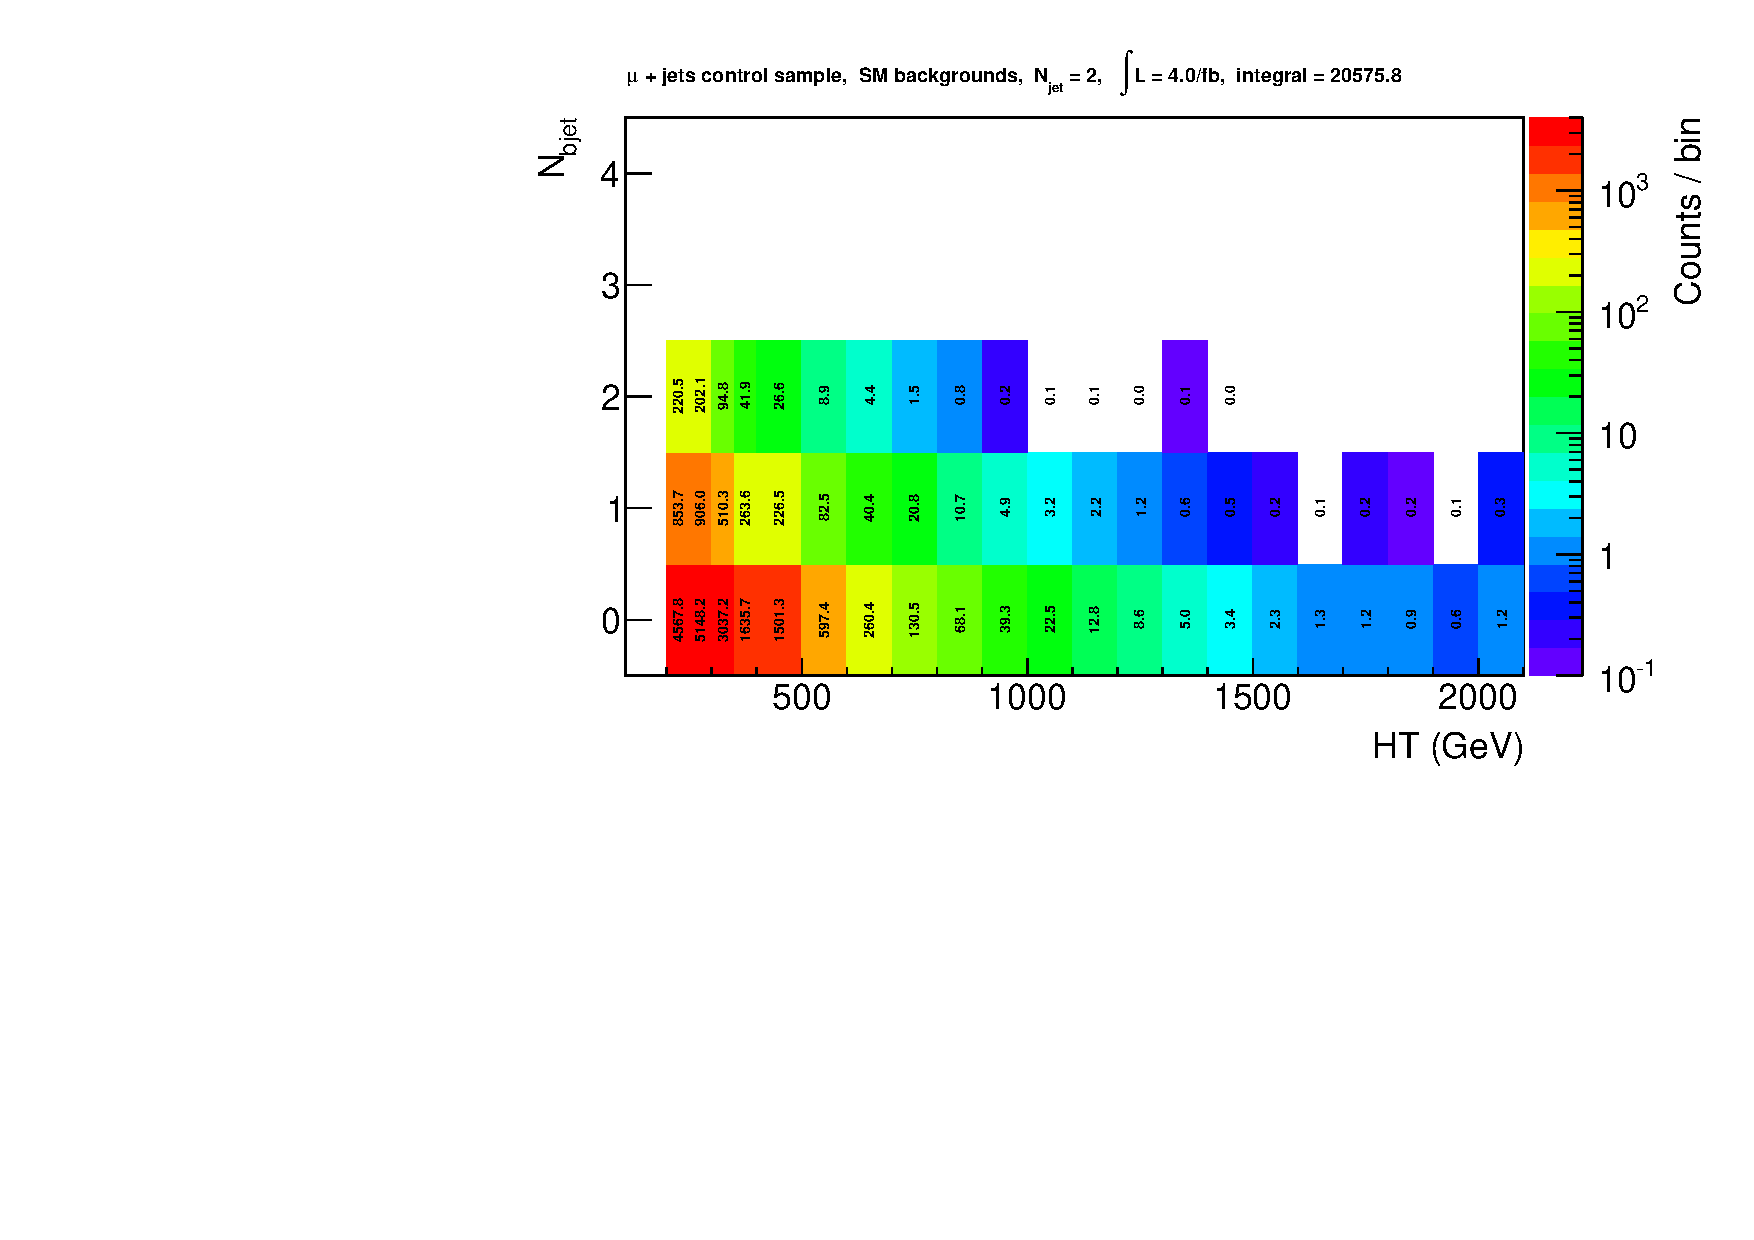
\includegraphics[width=0.5\textwidth]{figures/yieldPlots/mu_ewk_eq2j.pdf}
  }~~
  \subfigure[Yields from \texorpdfstring{\mj}{muon plus jets} control sample
  ($\njet = 3$)]{
    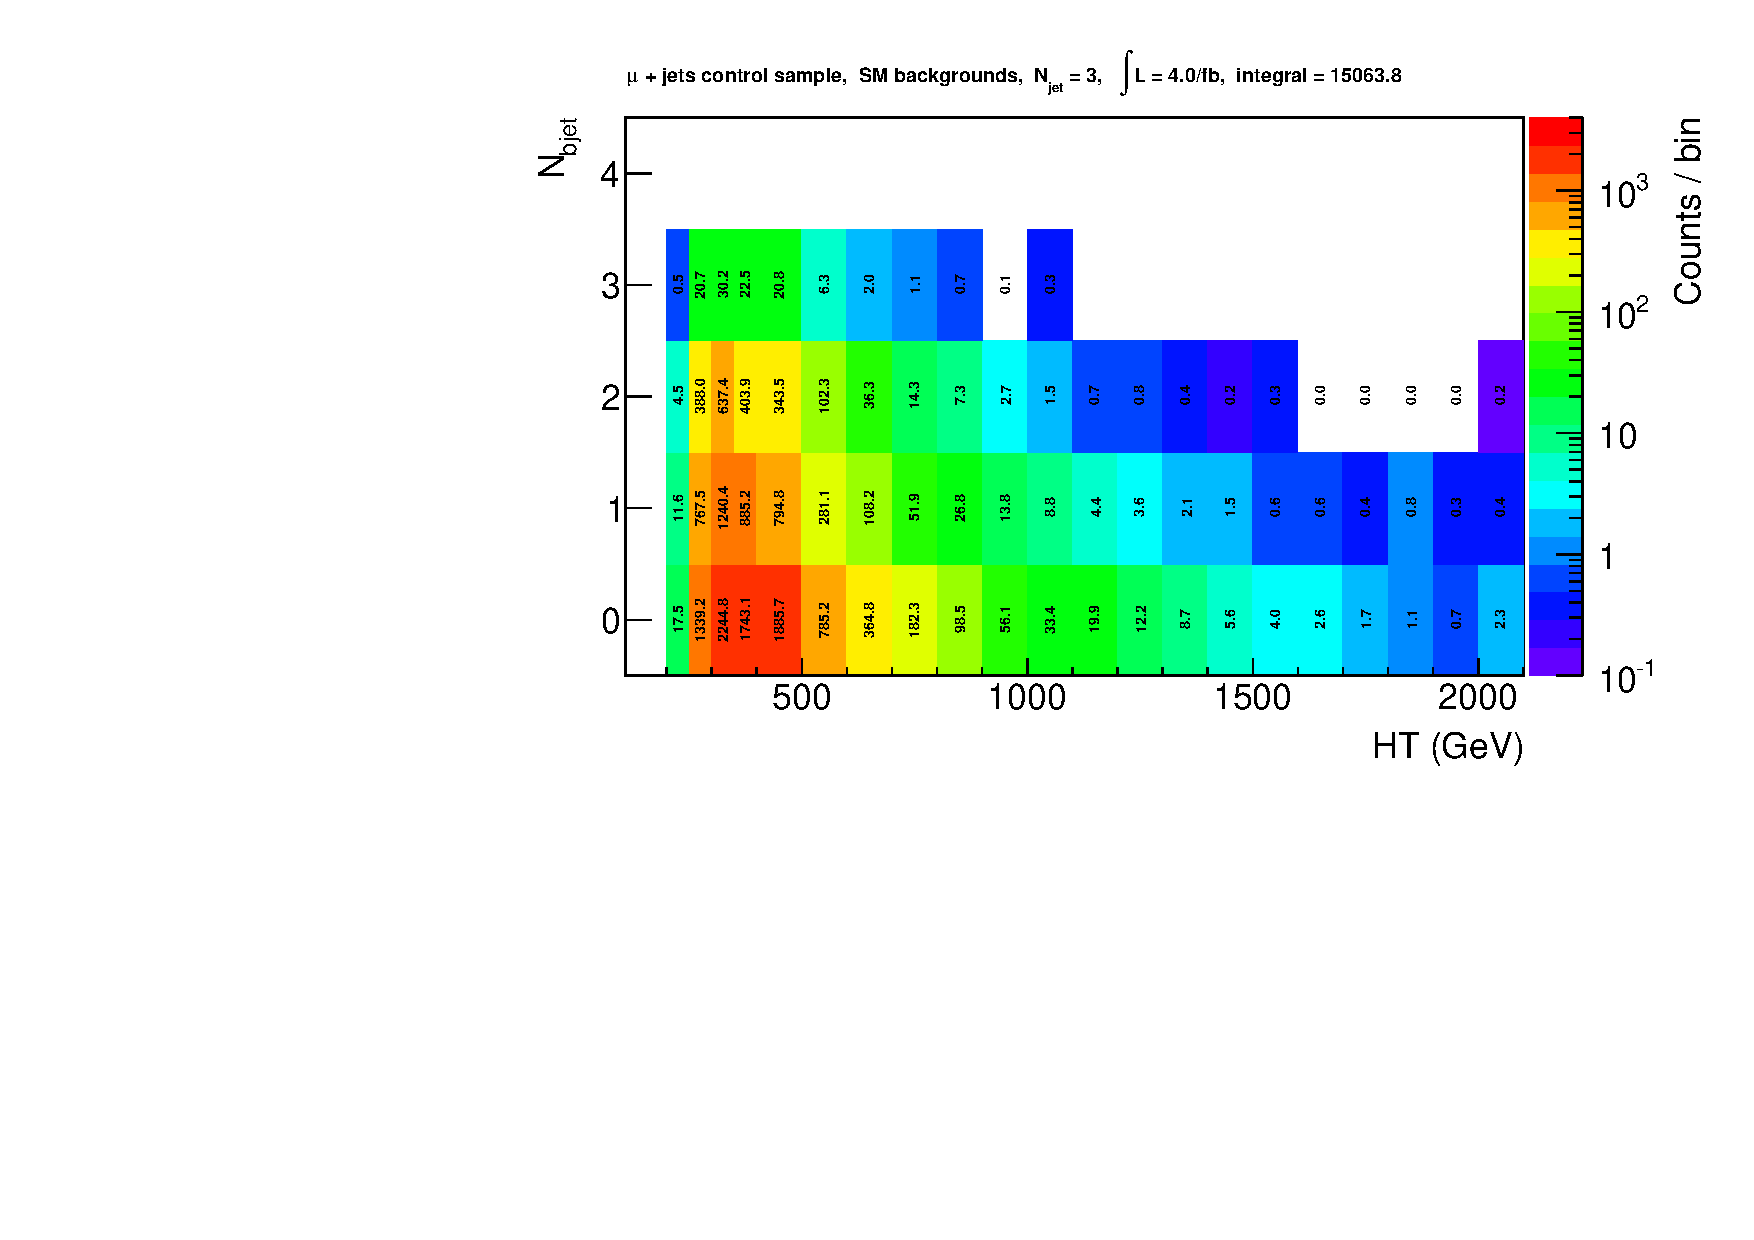
\includegraphics[width=0.5\textwidth]{figures/yieldPlots/mu_ewk_eq3j.pdf}
  }
  \\
  \subfigure[Yields from \texorpdfstring{\mj}{muon plus jets} control sample
  ($\njet = 4$)]{
    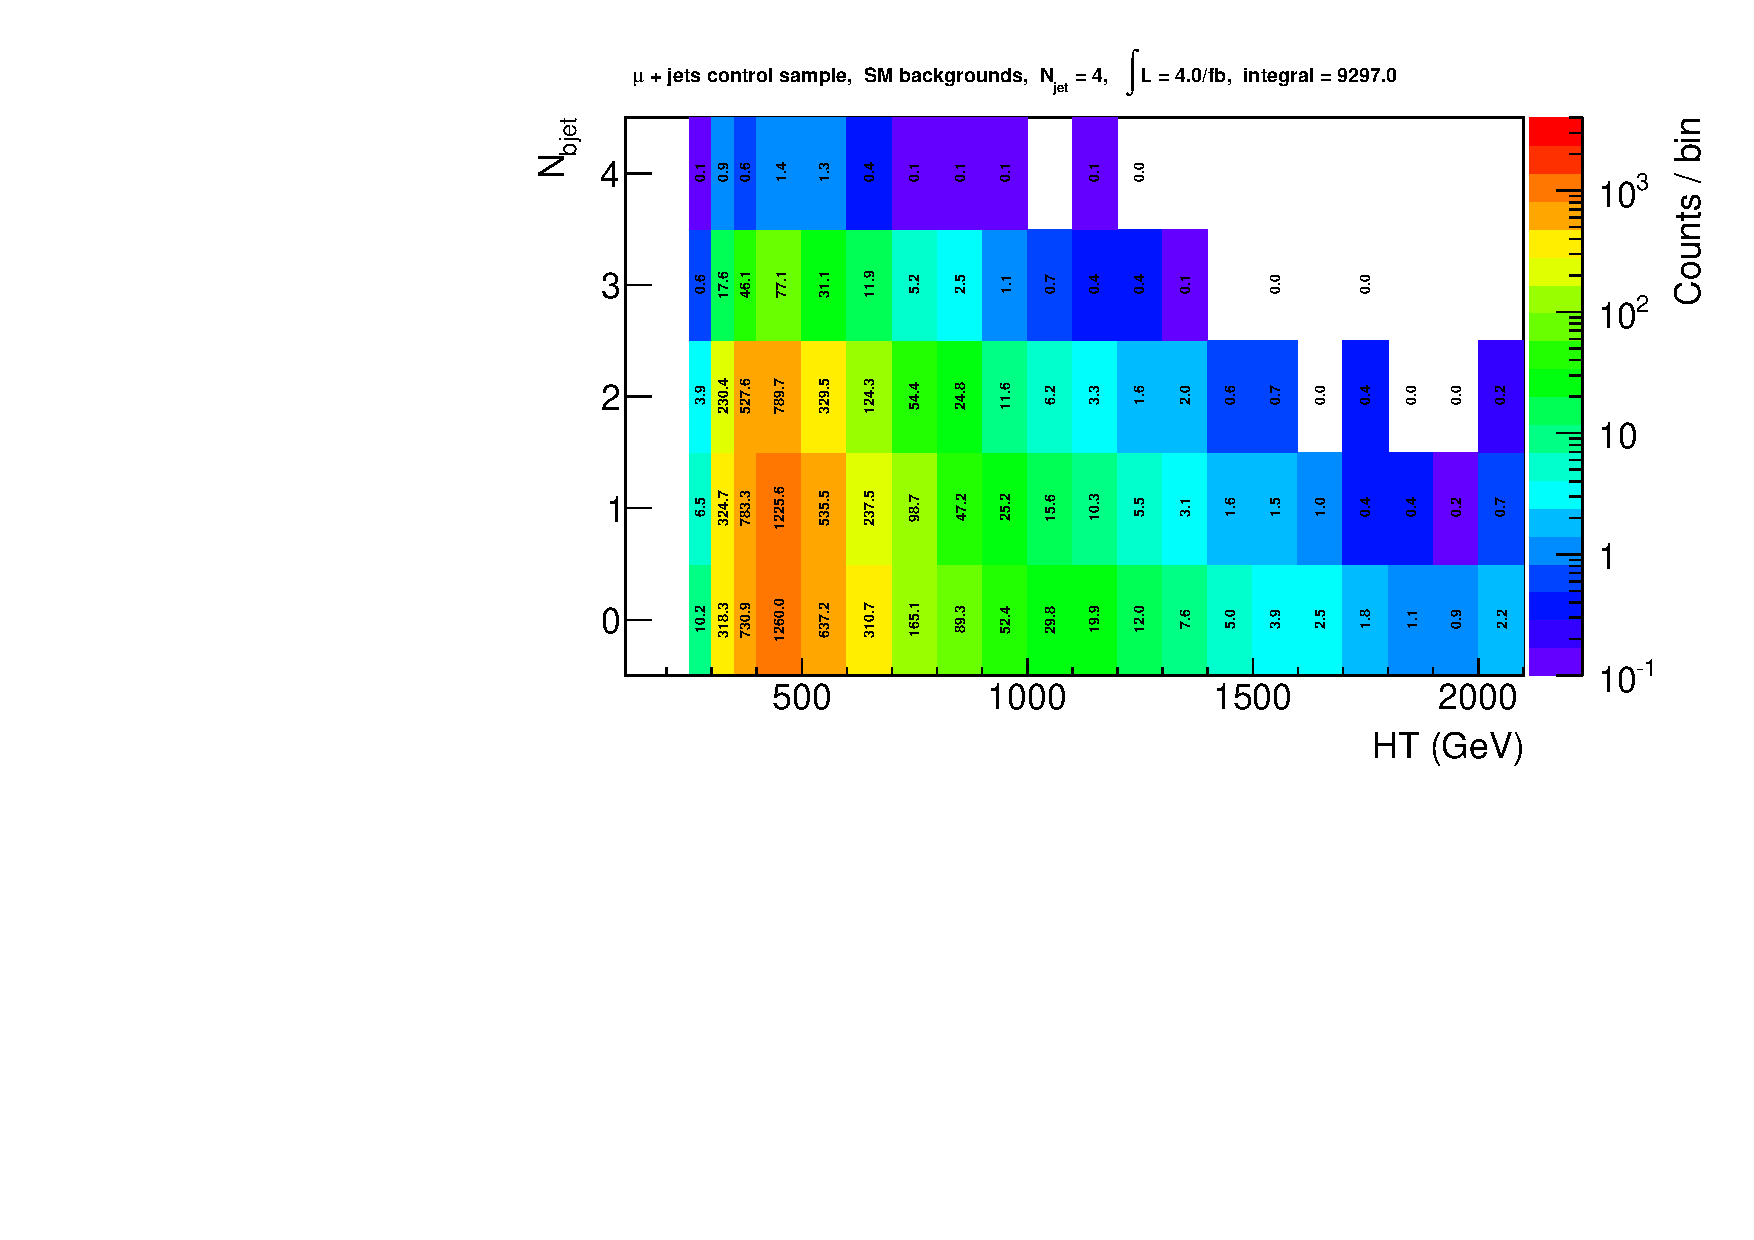
\includegraphics[width=0.5\textwidth]{figures/yieldPlots/mu_ewk_eq4j.pdf}
  }~~
  \subfigure[Yields from \texorpdfstring{\mj}{muon plus jets} control sample
  ($\njet \geq 5$)]{
    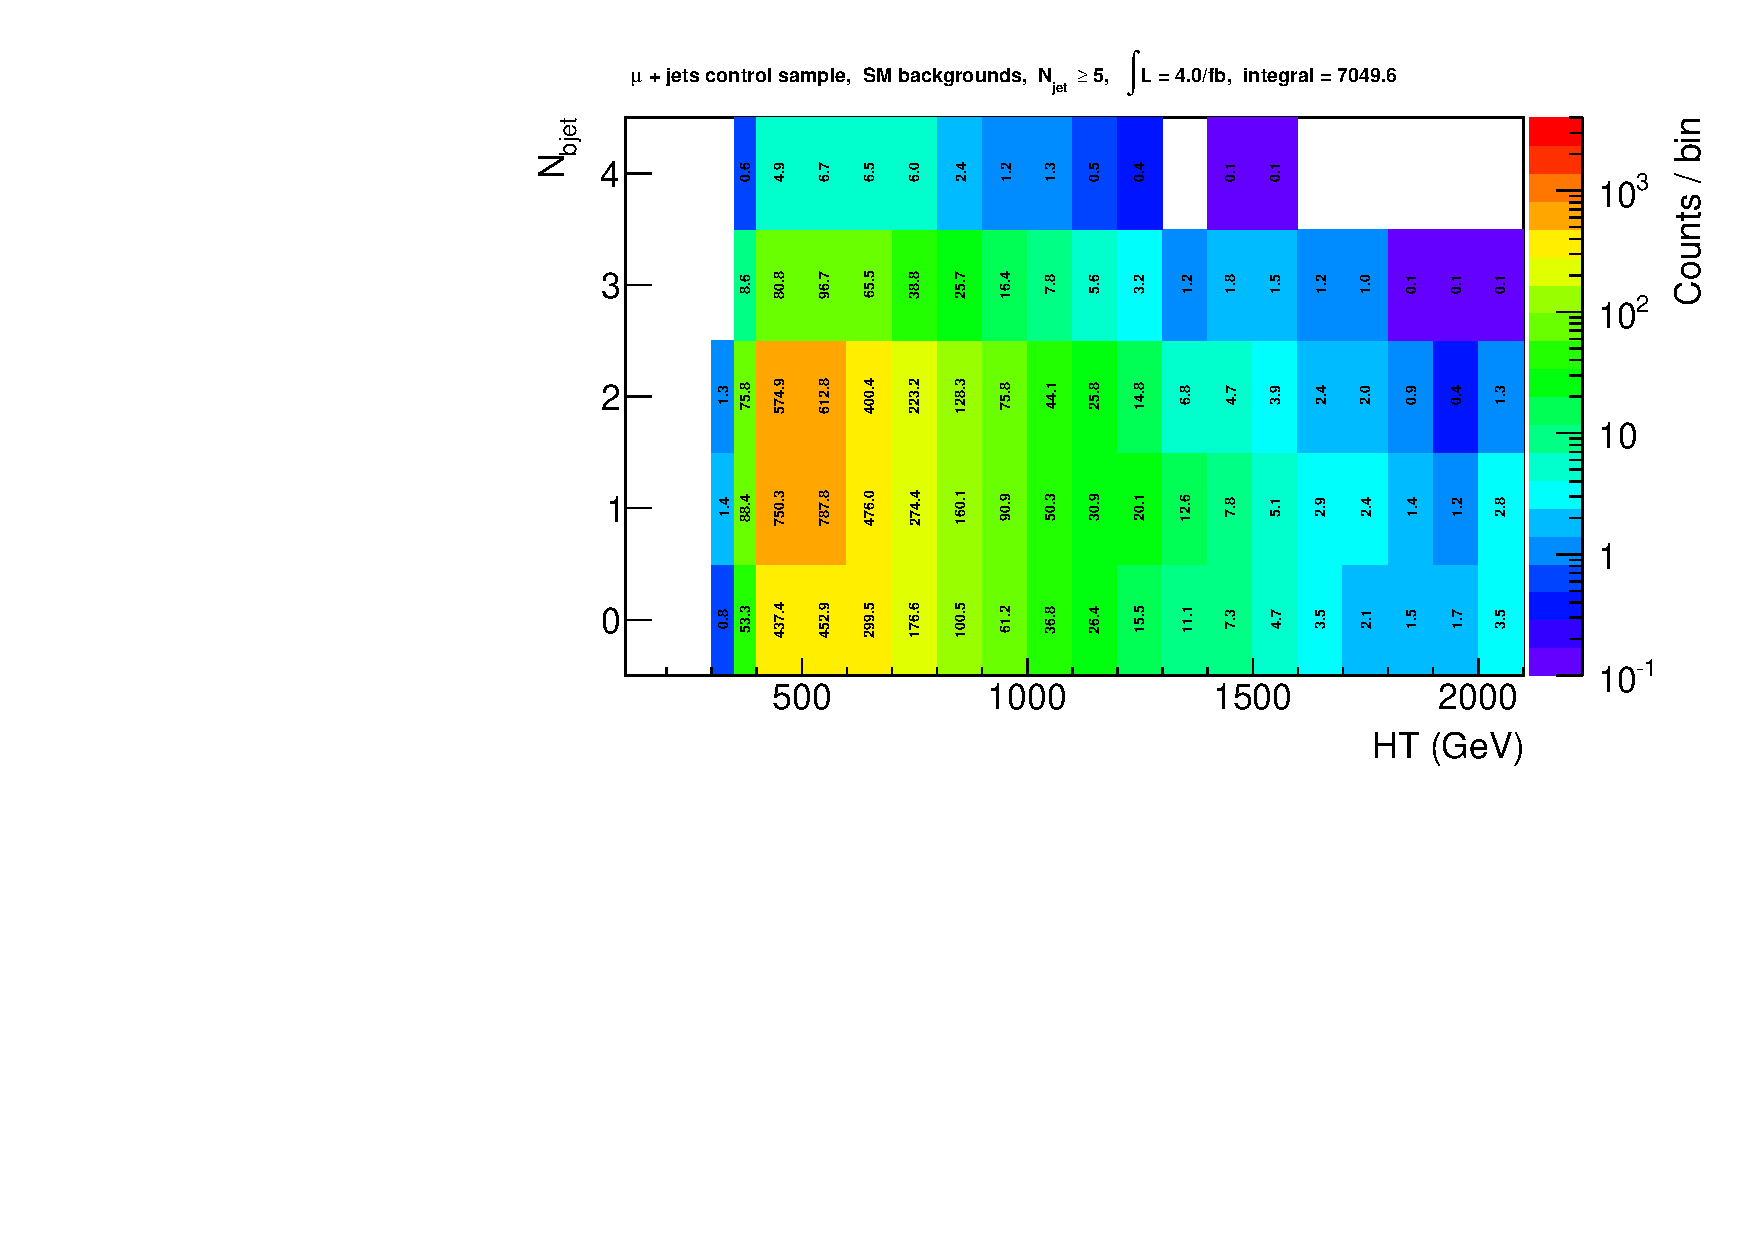
\includegraphics[width=0.5\textwidth]{figures/yieldPlots/mu_ewk_ge5j.pdf}
  } 
  \\
  \caption{\label{fig:ewkYields} Yields at $4\fbinv$ for the W~+~jets and \ttbar
  MC contributions to the \texorpdfstring{\mj}{muon plus jets} control sample. }
\end{figure}


\subsubsection{The \texorpdfstring{\mmj}{di-muon plus jets} control sample}

The \znunu\ + jets process forms an irreducible background and can be
estimated using the \zmumu + jets process, which has similar kinematic
properties but a different acceptance and a smaller branching ratio. A
background estimate is obtained through the use of a \mmj sample. Most
of the selection criteria are identical to those for the \mj sample,
but the few that differ are tuned to identify Z bosons decaying to two
muons in the kinematic phase space of the signal region. The muons are
not considered in the calculation of event-level variables such as
\scalht, \mht and \alphat. All cuts on such jet-based quantities are
consistent with those applied in the hadronic search region and the
same \njet, \nb, and \scalht binning is used. The only exception is
that no \alphat requirement is made, as motivated by the discussion in
Sec.~\ref{sec:larger}. In order to select an event sample containing Z
bosons, exactly two tight isolated muons within an acceptance of $\Pt
> 30\gev$ and $|\eta| < 2.1$ are required (due to the trigger). The
invariant mass of the two muons must satisfy $m_{Z} - 25 <
M_{\mu_1\mu_2} < m_{Z} + 25$. Events are vetoed if $\Delta
R(\mu_{i},\textrm{jet}_j) < 0.5$ is satisfied, running over all muons
$i$ and all jets $j$. The single isolated track veto, described in
Sections~\ref{sec:reconstruction} and~\ref{sec:vetoes}, is also
applied, considering all single isolated tracks in the event except
those associated with the two identified, isolated muons. Finally, the
cleaning cut $\mht/\pfmet$ is also applied, as done in the signal
region, where the \pfmet is adjusted to account for the transverse
momenta of the two identified, isolated muons. The \mmj sample can be
used to make predictions in all the \scalht bins, providing coverage
at low \scalht where the \gj sample cannot.

\begin{figure}[h!]
  \centering
  \subfigure[Yields from \texorpdfstring{\mmj}{di-muon plus jets} control sample
  ($\njet = 2$)]{
    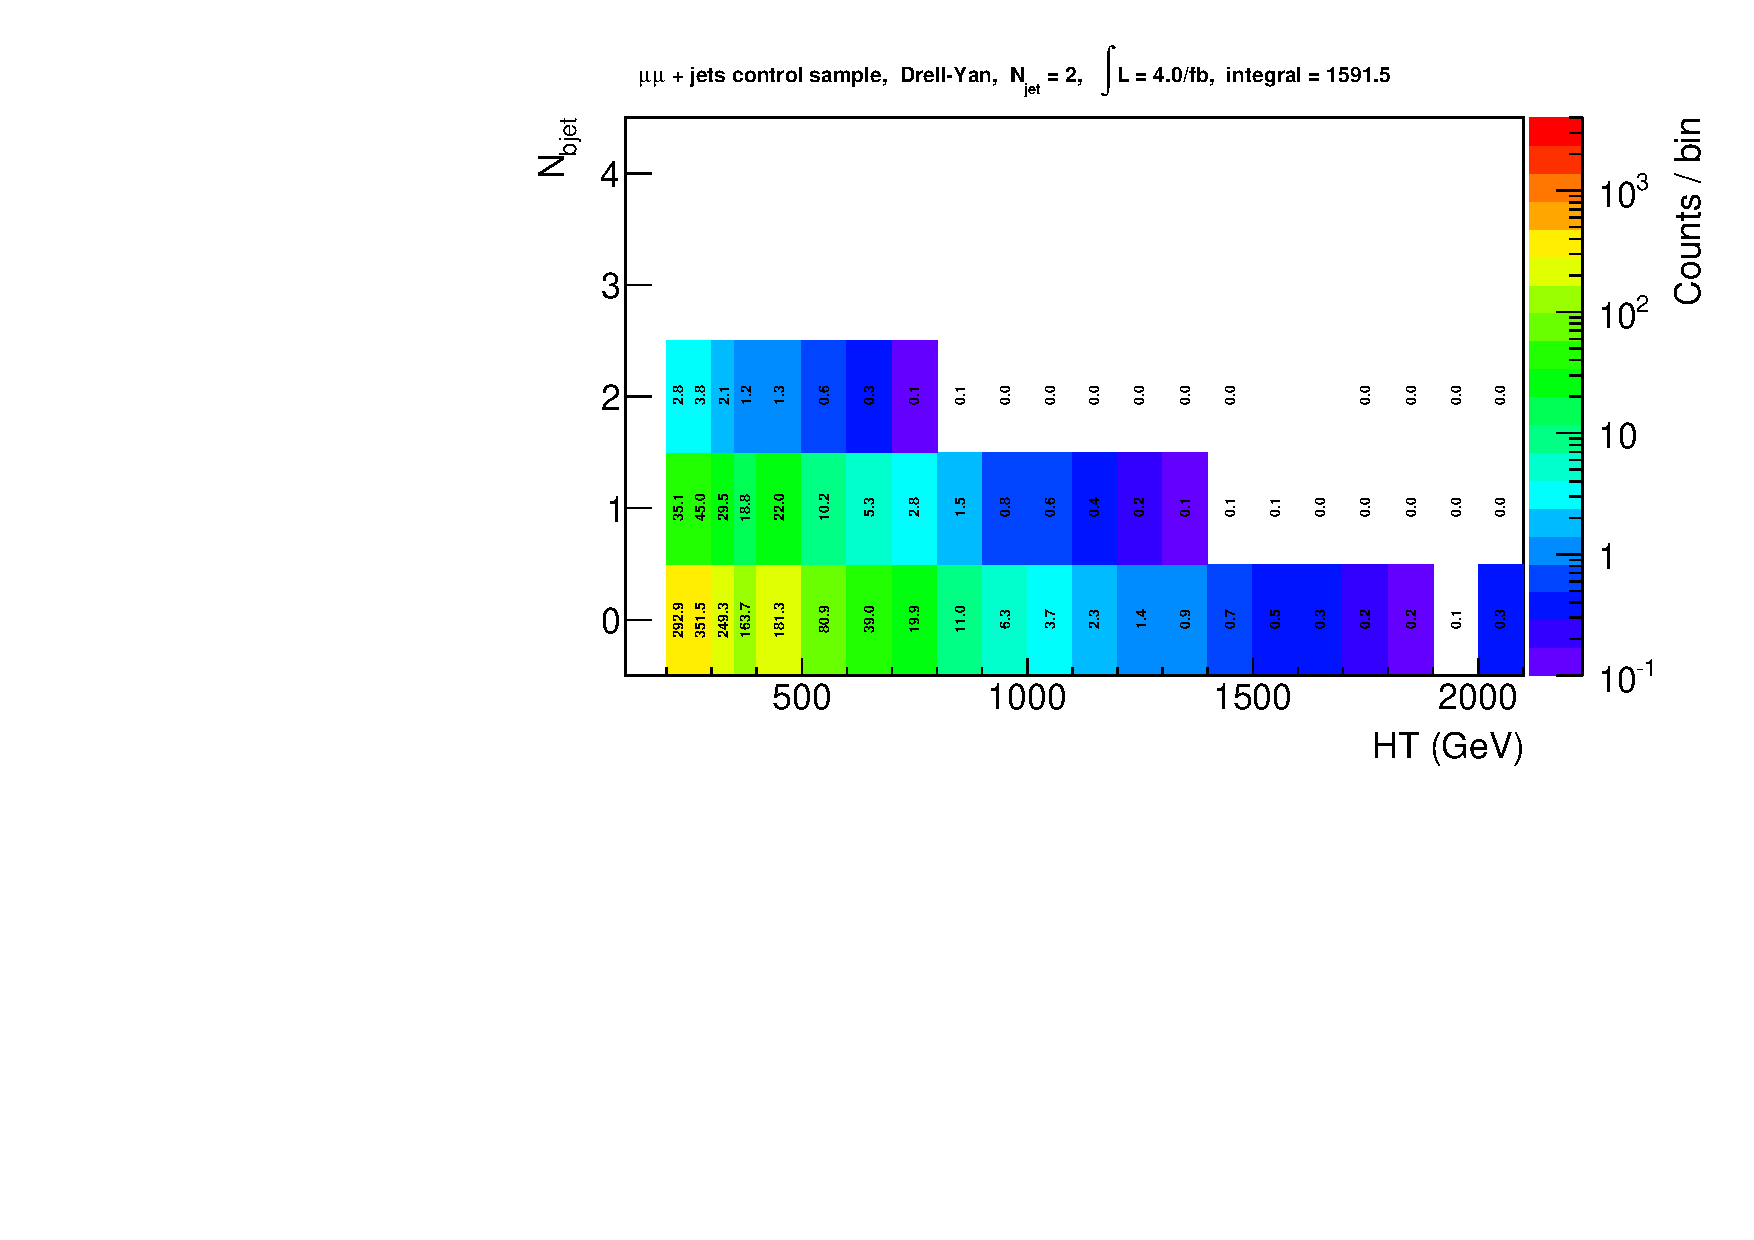
\includegraphics[width=0.5\textwidth]{figures/yieldPlots/mm_dy_eq2j.pdf}
  }~~
  \subfigure[Yields from \texorpdfstring{\mmj}{di-muon plus jets} control sample
  ($\njet = 3$)]{
    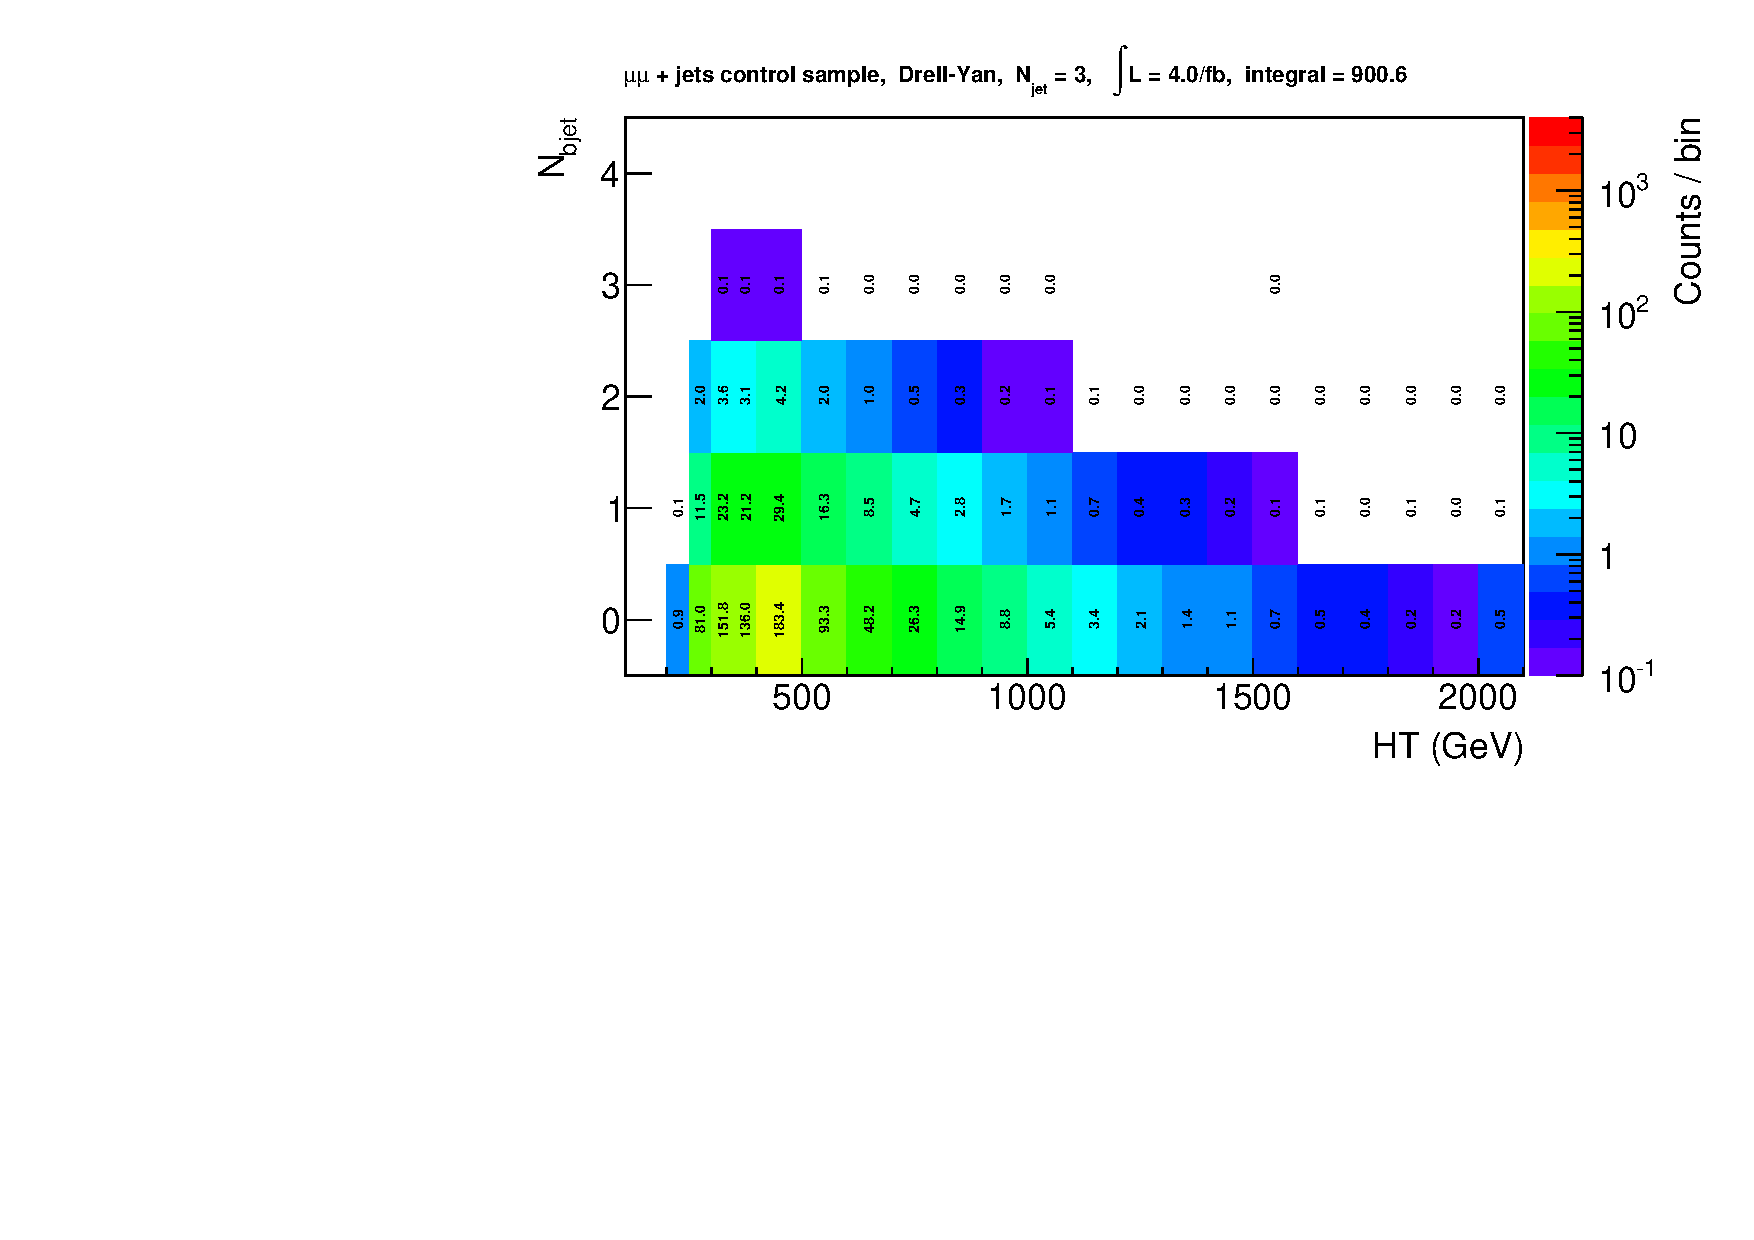
\includegraphics[width=0.5\textwidth]{figures/yieldPlots/mm_dy_eq3j.pdf}
  }
  \\
  \subfigure[Yields from \texorpdfstring{\mmj}{di-muon plus jets} control sample
  ($\njet = 4$)]{
    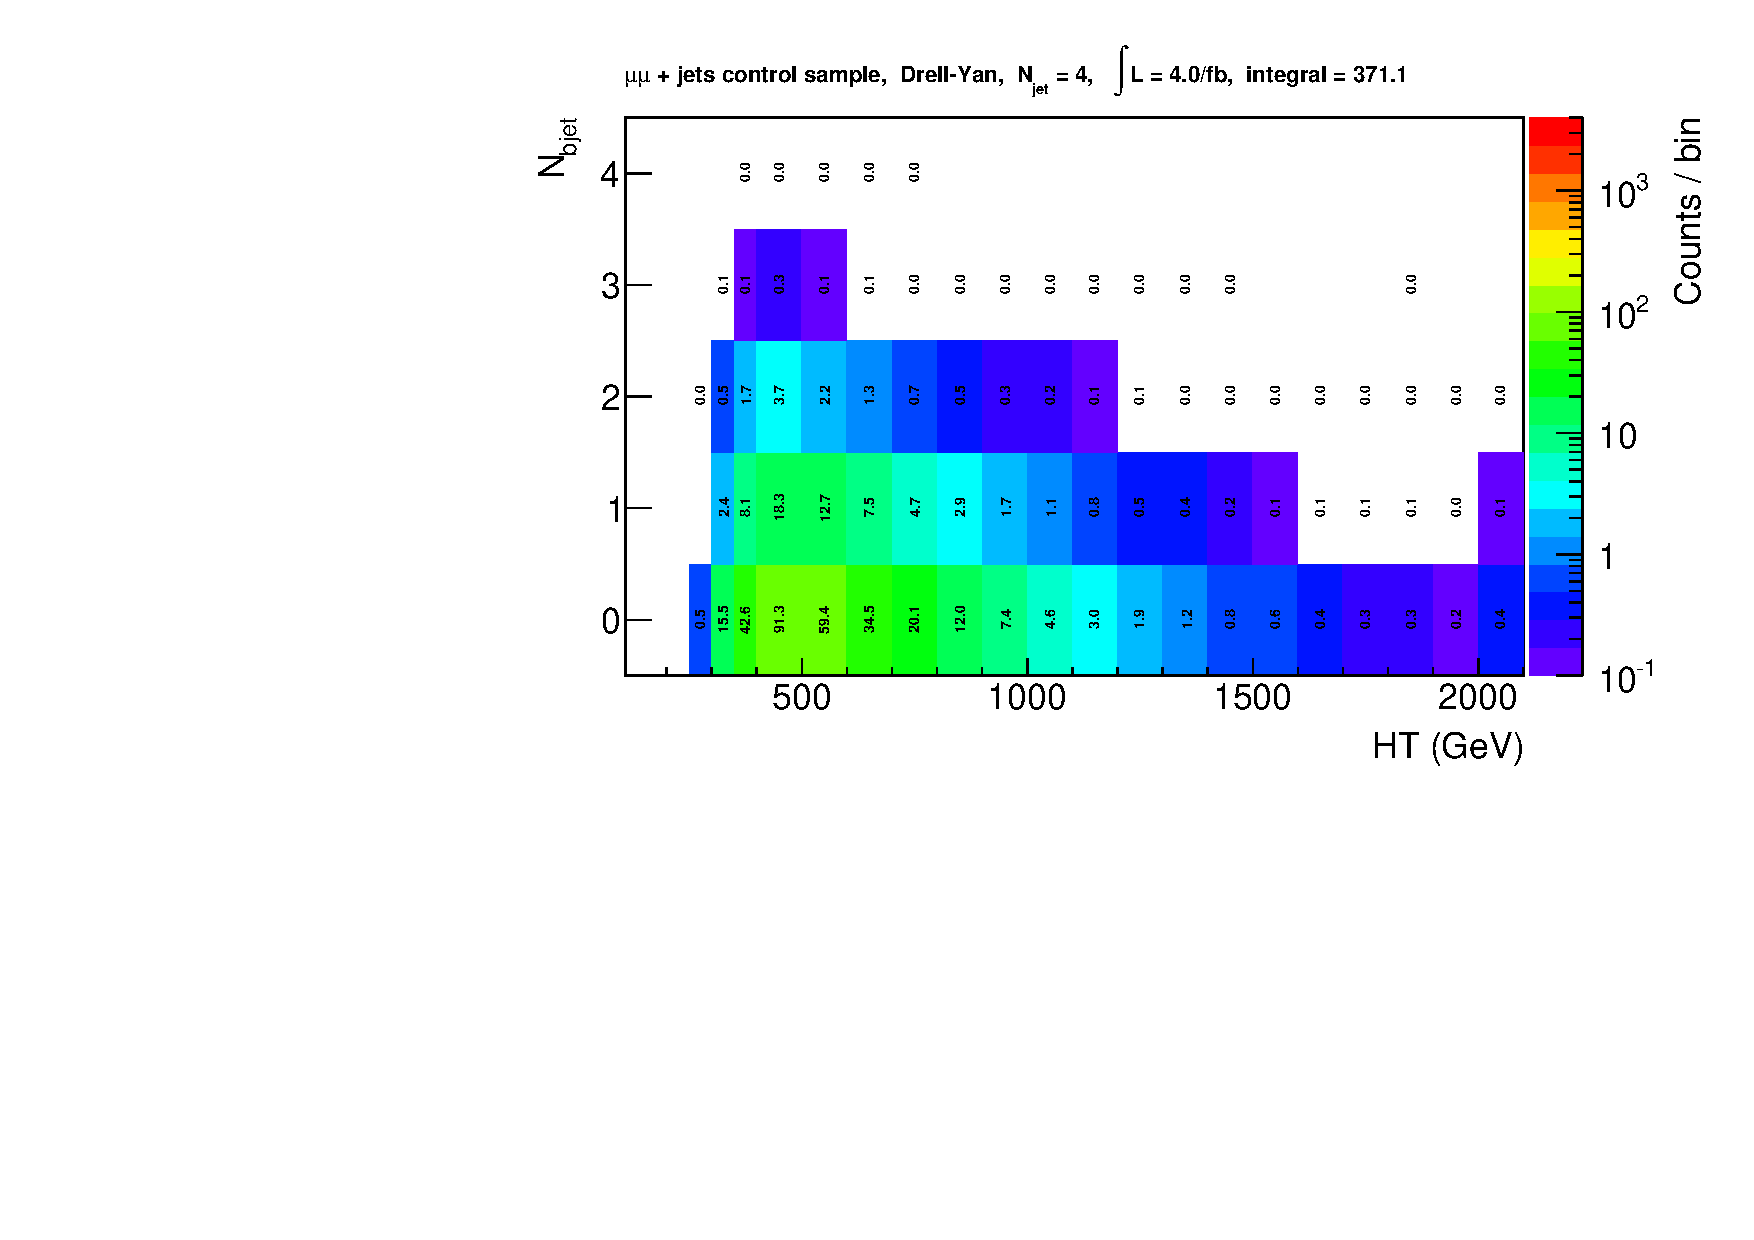
\includegraphics[width=0.5\textwidth]{figures/yieldPlots/mm_dy_eq4j.pdf}
  }~~
  \subfigure[Yields from \texorpdfstring{\mmj}{di-muon plus jets} control sample
  ($\njet \geq 5$)]{
    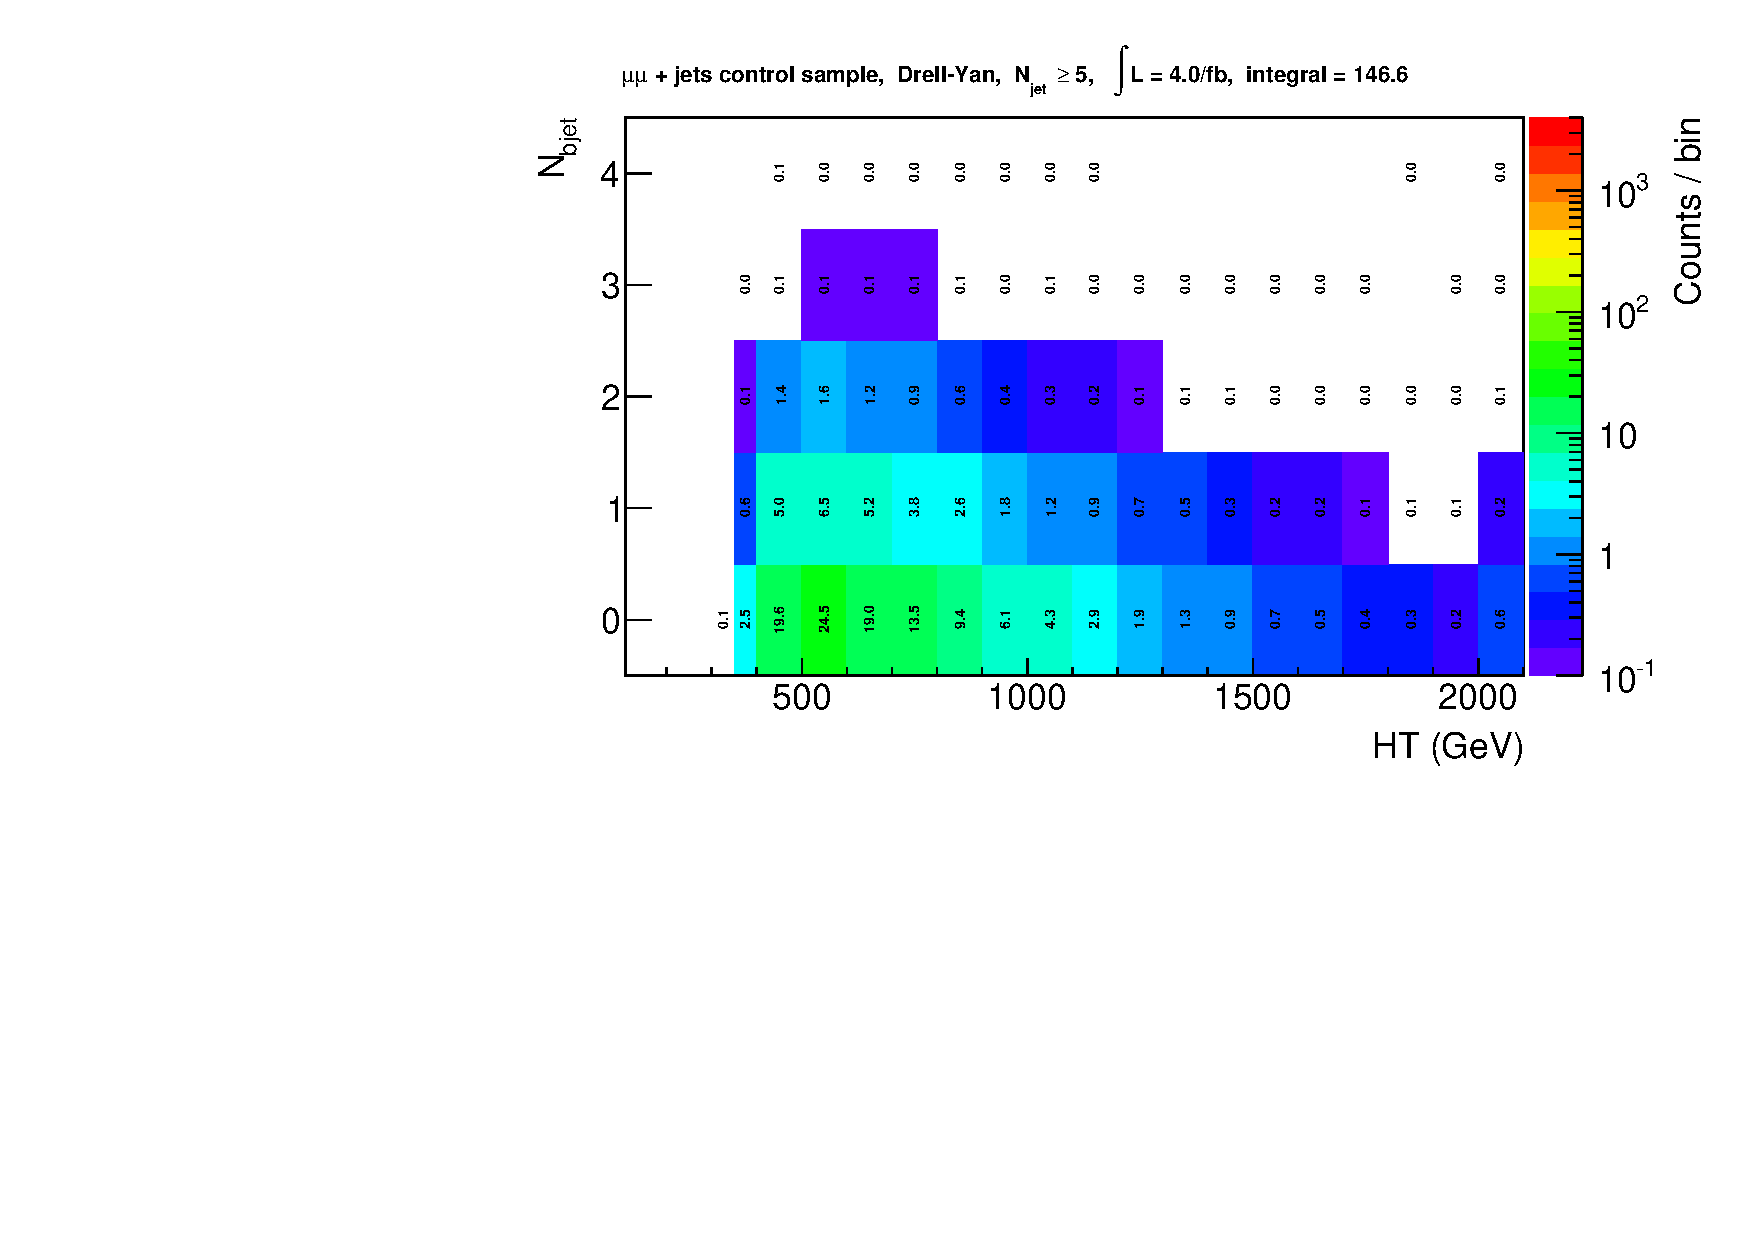
\includegraphics[width=0.5\textwidth]{figures/yieldPlots/mm_dy_ge5j.pdf}
  } 
  \\
  \caption{\label{fig:ewkYields} Yields at $4\fbinv$ for the DY~+~jets MC 
  contributions to the \texorpdfstring{\mmj}{di-muon plus jets} control sample. }
\end{figure}

\subsubsection{The \texorpdfstring{\gj}{photon plus jets} control sample}

The \znunu\ + jets process can also be estimated using the \gj
process, which has a larger cross section and kinematic properties
similar to those of \znunu\ events when the photon is
ignored~\cite{PAS-SUS-08-002,Bern:2011pa}. The \gj sample is defined
by requiring exactly one photon satisfying tight isolation criteria
and within an acceptance of $\pt > 175\gev$ and $|\eta| <
1.45$ (the anticipated limitation from the trigger). Furthermore, events are vetoed if $\Delta
R(\gamma,\textrm{jet}_j) < 1.0$ is satisfied, running over all jets
$j$. As for the muon-based samples, the photon is not considered in
the calculation of event-level variables such as \scalht, \mht, \met and 
\alphat. All cuts on jet-based quantities are consistent with those
applied in the hadronic search region, and the same \HT binning is
used. 
% Given that the photon is ignored, the \gj sample can only be
% used for the region $\scalht > 375\gev$ due to the photon acceptance
% of $\pt > 165\gev$ (enforced by the trigger) and the requirement
% $\alphat > 0.55$.

\begin{figure}[h!]
  \centering
  \subfigure[Yields from \texorpdfstring{\gj}{photon plus jets} control sample
  ($\njet = 2$)]{
    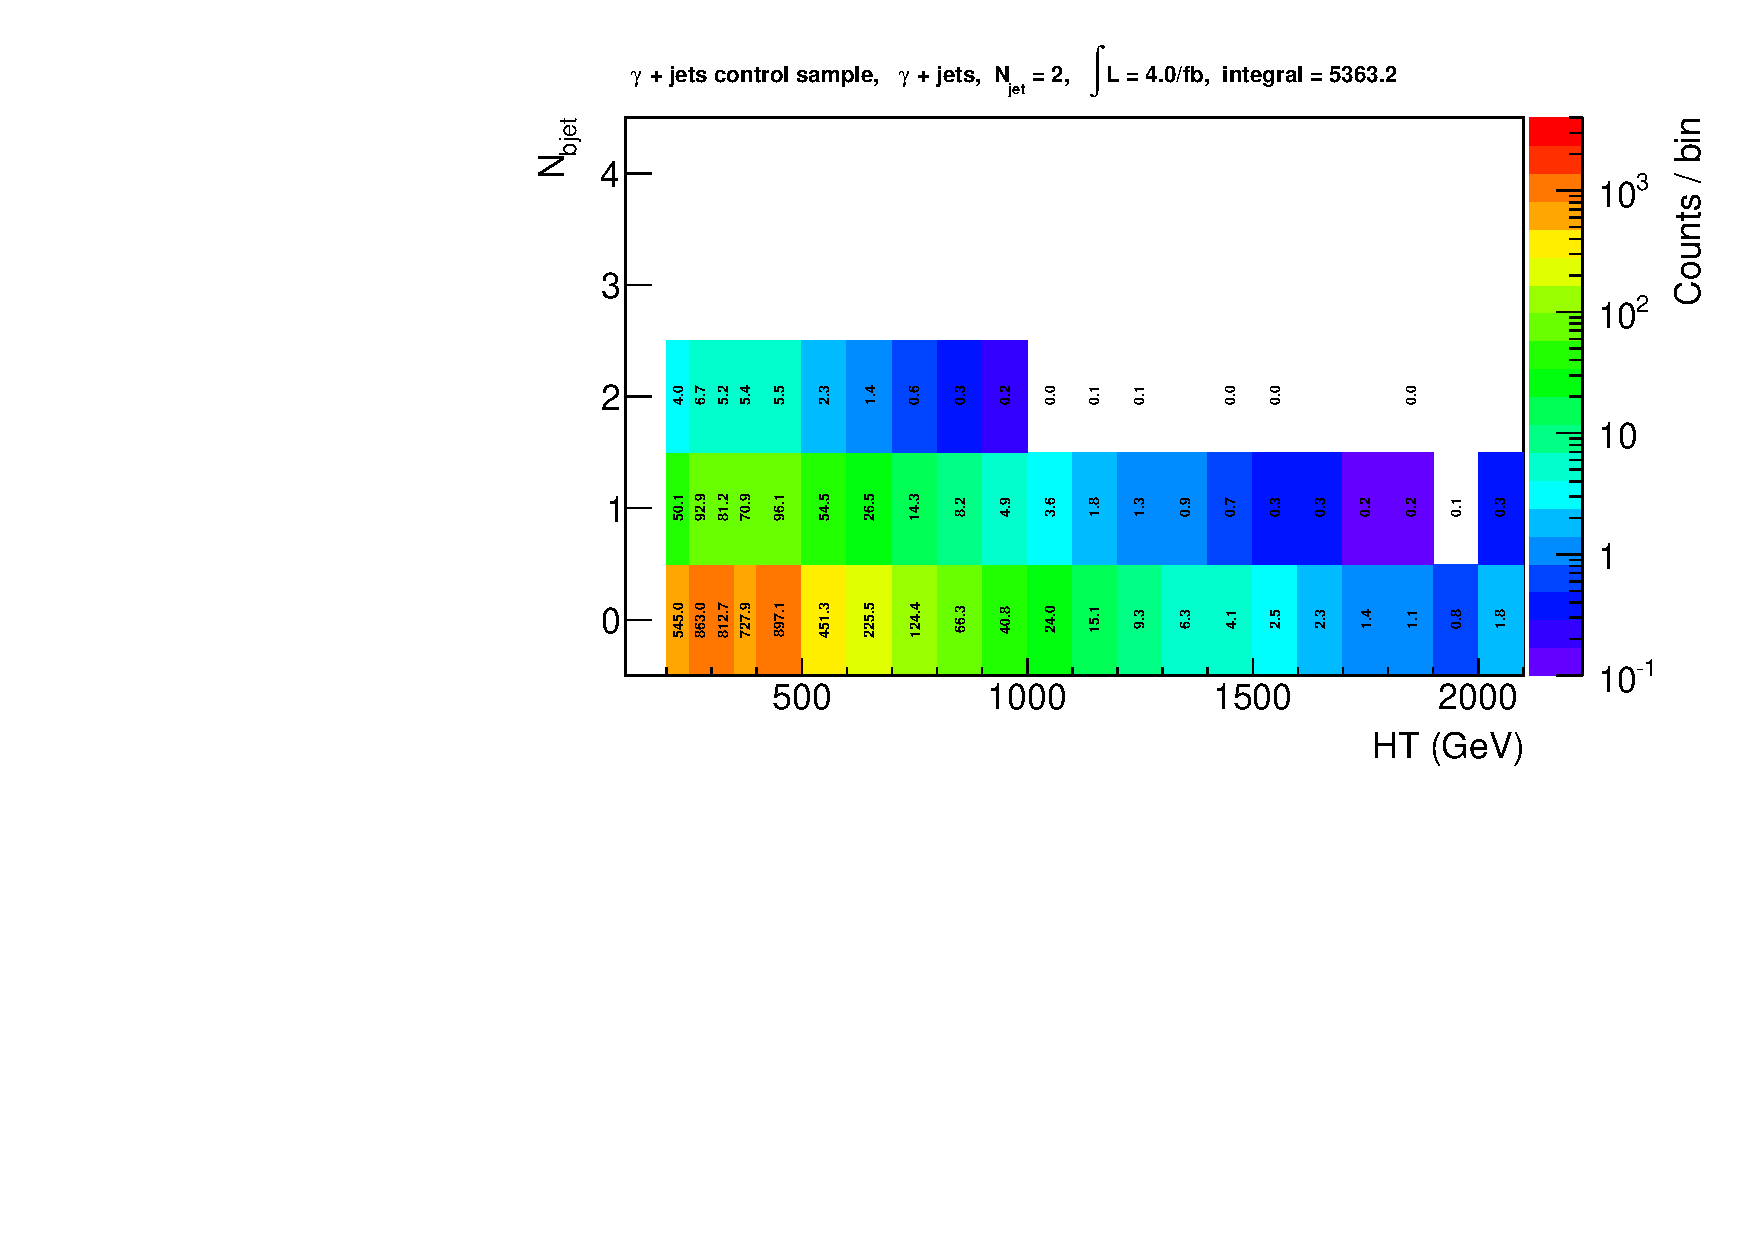
\includegraphics[width=0.5\textwidth]{figures/yieldPlots/ph_gjets_eq2j.pdf}
  }~~
  \subfigure[Yields from \texorpdfstring{\gj}{photon plus jets} control sample
  ($\njet = 3$)]{
    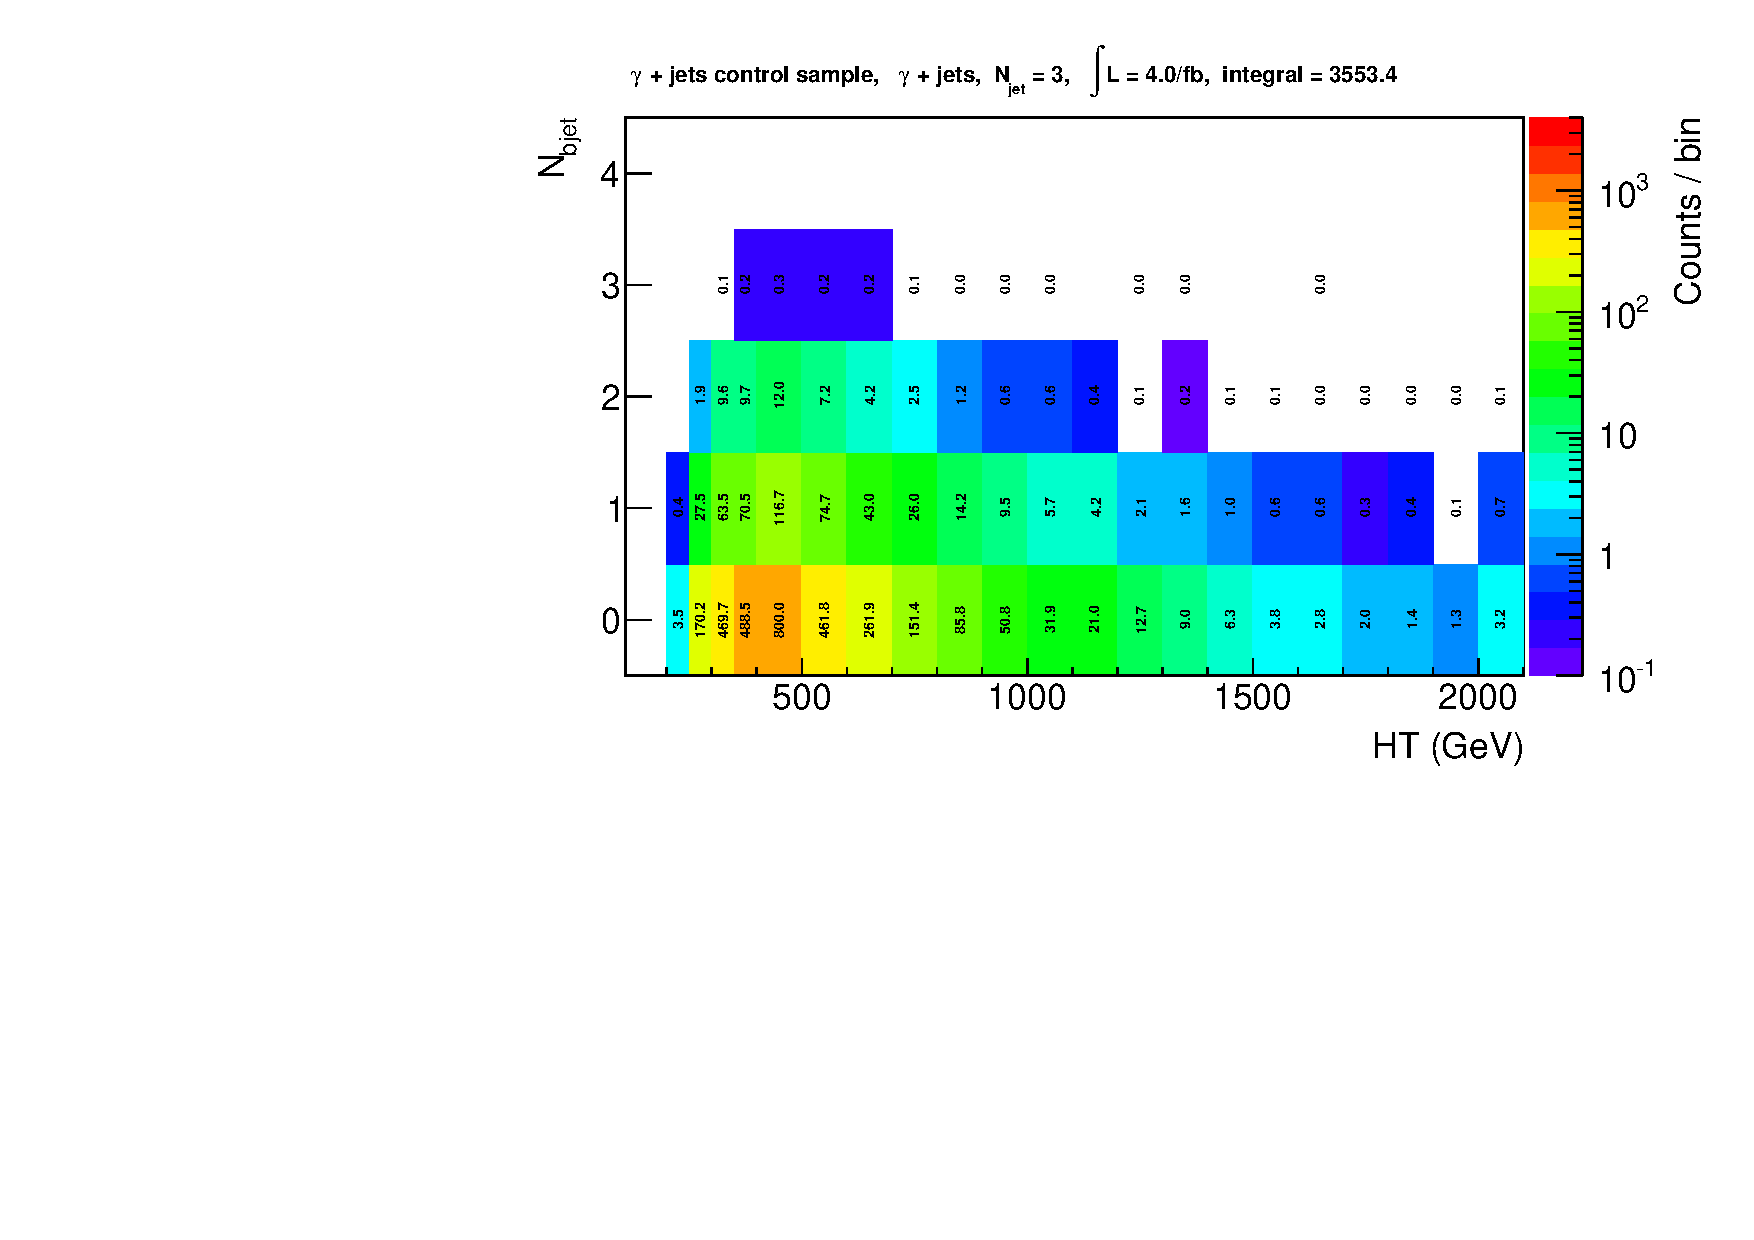
\includegraphics[width=0.5\textwidth]{figures/yieldPlots/ph_gjets_eq3j.pdf}
  }
  \\
  \subfigure[Yields from \texorpdfstring{\gj}{photon plus jets} control sample
  ($\njet = 4$)]{
    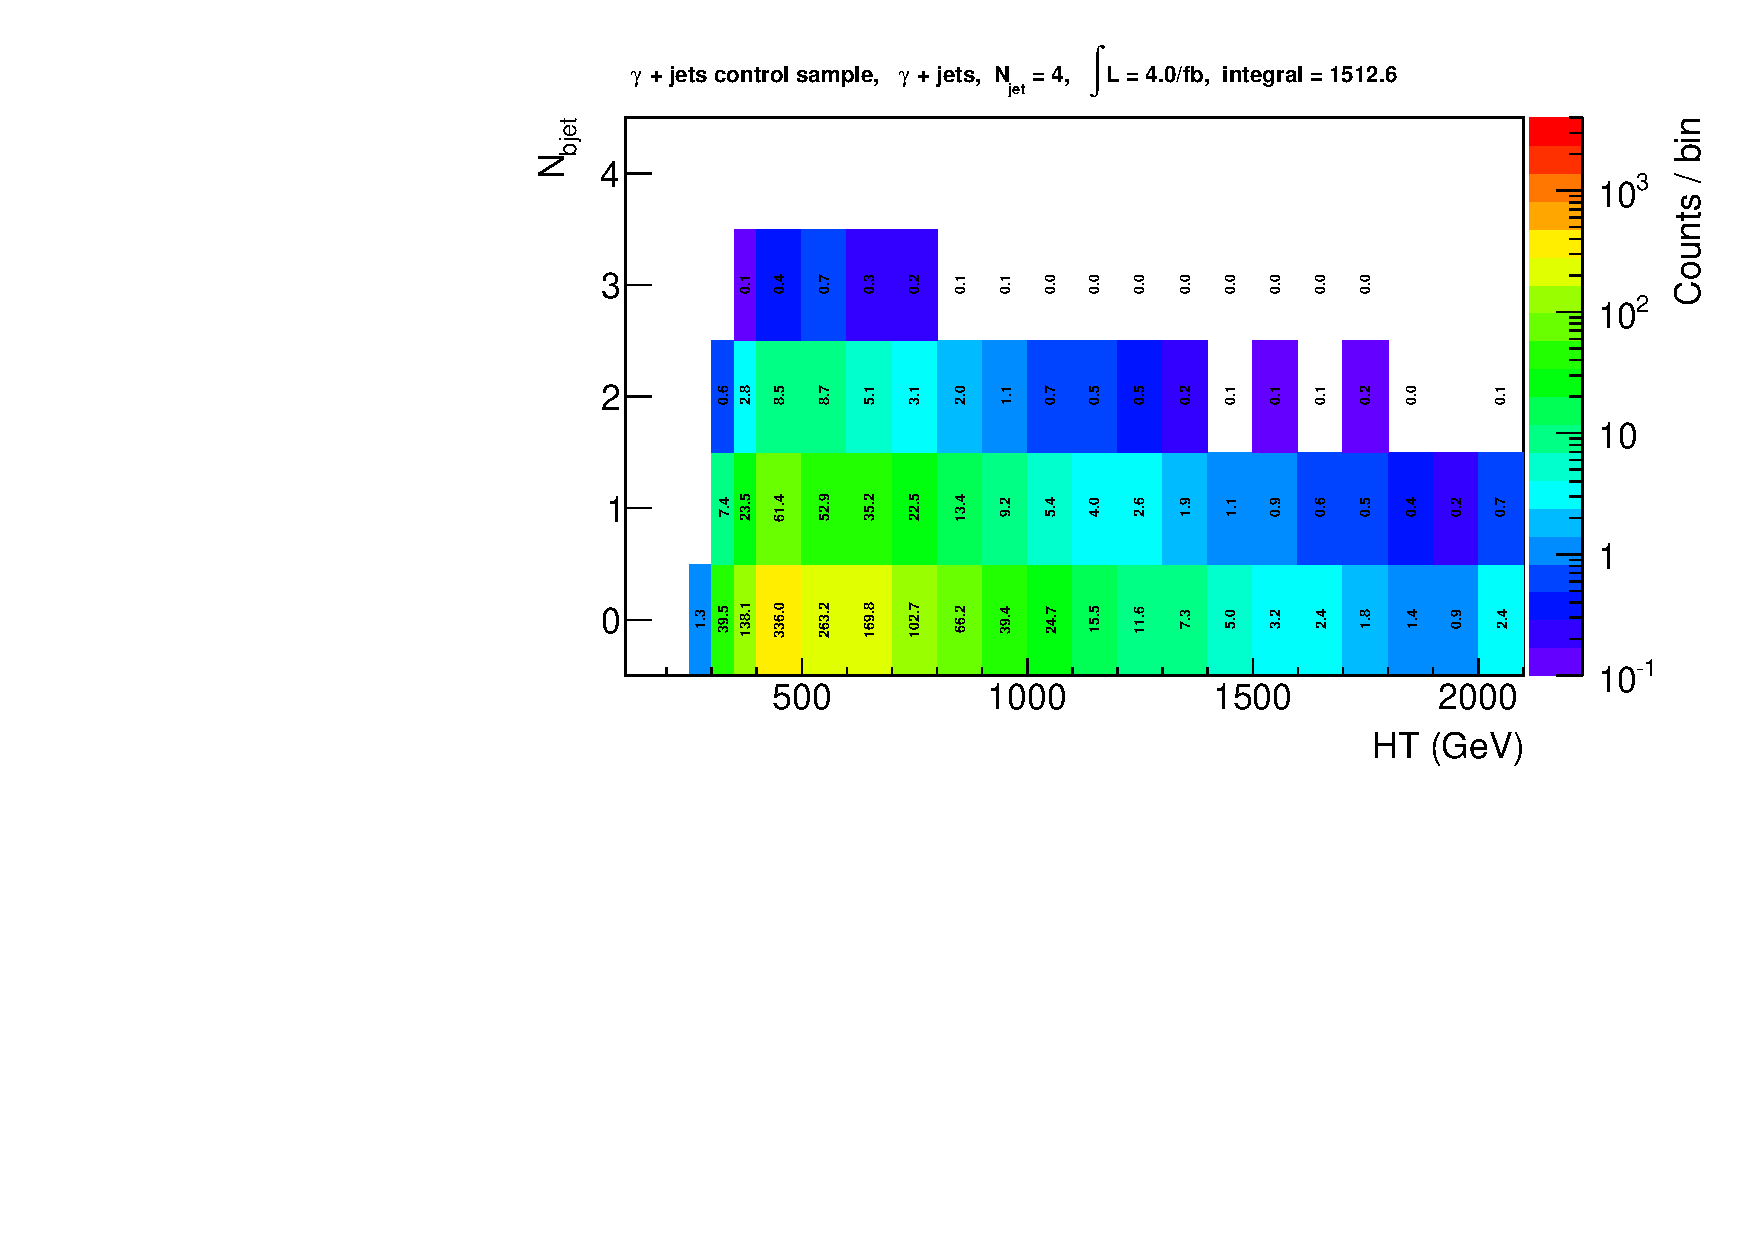
\includegraphics[width=0.5\textwidth]{figures/yieldPlots/ph_gjets_eq4j.pdf}
  }~~
  \subfigure[Yields from \texorpdfstring{\gj}{photon plus jets} control sample
  ($\njet \geq 5$)]{
    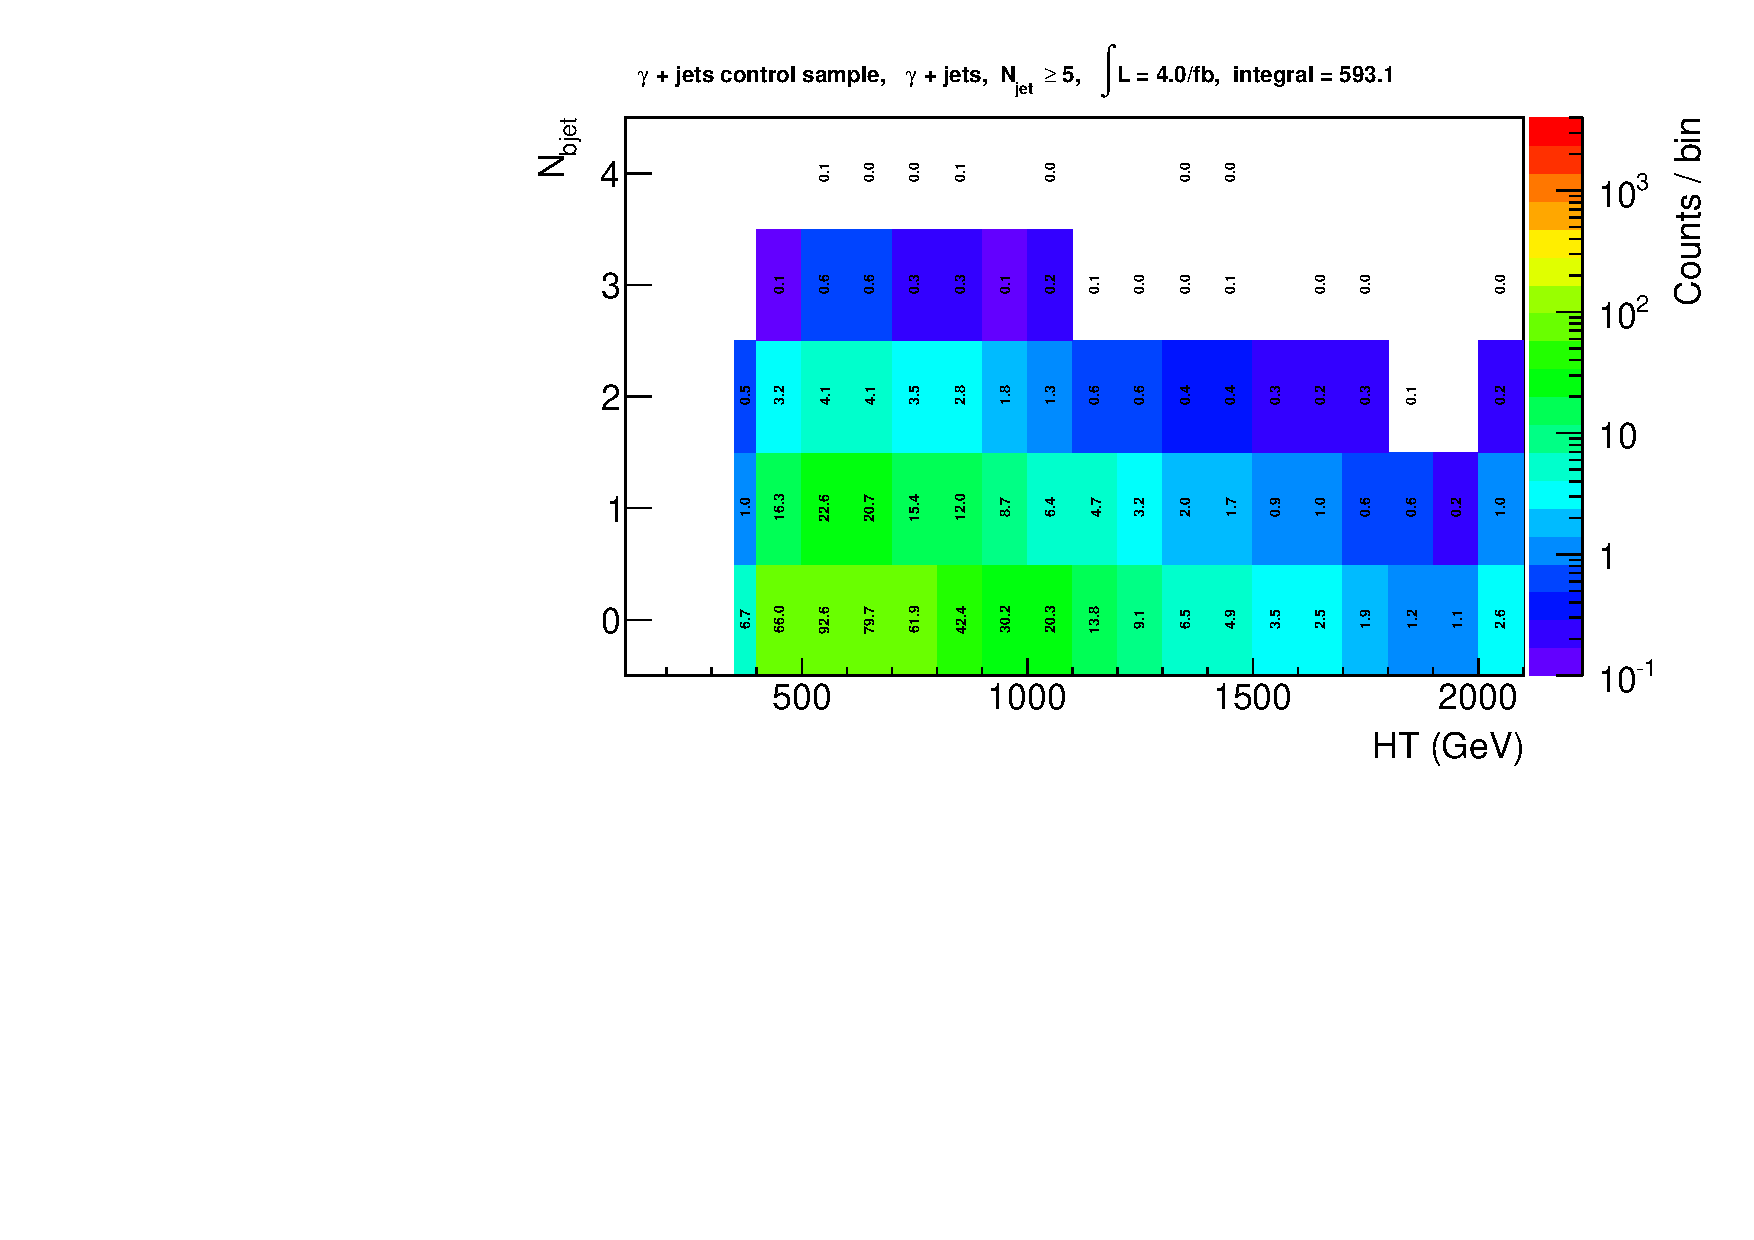
\includegraphics[width=0.5\textwidth]{figures/yieldPlots/ph_gjets_ge5j.pdf}
  } 
  \\
  \caption{\label{fig:ewkYields} Yields at $4\fbinv$ for the \gamma~+~jets MC 
  contributions to the \texorpdfstring{\gj}{photon plus jets} control sample. }
\end{figure}


%%____________________________________________________________________________||
\subsection{Future developments in the acceptance of the control samples\label{sec:larger}}
EGM-14-001 - tight to medium
%Add electron control sample

%%____________________________________________________________________________||
